% --- Empiezan las configuraciones ---------
\documentclass[11pt,a4paper,openright,oneside]{article}
%\usepackage{amsfonts, amsmath, amssymb,latexsym,amsthm, mathrsfs, enumerate, tikz-cd}
\usepackage{amsfonts, amsmath, amssymb,latexsym,amsthm, mathrsfs, enumerate, tikz-cd}

\usepackage[all]{xy}

\SelectTips{cm}{} %to change the tips and tail of the arrows 
% \usepackage[spanish]{babel}
\usepackage{epsfig}

\parskip=5pt
\parindent=15pt
\usepackage[margin=1.2in]{geometry}
\usepackage{graphicx}
\usepackage{listings}
\usepackage[latin1]{inputenc}
\usepackage{fancyhdr}

\setcounter{page}{0}


\numberwithin{equation}{section}
\newtheorem{teo}{Teorema}[section]
\newtheorem*{teo*}{Teorema}
\newtheorem{prop}[teo]{Proposici\'on}
\newtheorem{corol}[teo]{Corolario}
\newtheorem{lema}[teo]{Lema}
\newtheorem{nota}[teo]{Notaci\'on}

\theoremstyle{definition}
\newtheorem{defi}[teo]{Definici\'on}
\newtheorem{prob}[teo]{Problema}
\newtheorem*{sol}{Soluci\'on}
\newtheorem{ex}[teo]{Ejemplo}
\newtheorem{exs}[teo]{Ejemplos}
\newtheorem{obs}[teo]{Observaci\'on}
\newtheorem{obss}[teo]{Observaciones}

\def\qed{\hfill $\square$}

\renewcommand{\refname}{Bibliografia}


% Definiciones de funciones matemáticas

\newcommand{\Set}{\mathop{\rm Set}}
\newcommand{\Grp}{\mathop{\rm Grp}}
\newcommand{\Top}{\mathop{\rm Top}}
\newcommand{\Oper}{\mathop{\rm Oper}}

\lhead{}
\lfoot{}
\rhead{}
\cfoot{}
\rfoot{\thepage}
\begin{document}
\bibstyle{plain}
\thispagestyle{empty}
% --- Acaban las configuraciones -----------

% ------------------------------------------
% ------------------------------------------
% ------------------------------------------

% --- Empieza la portada -------------------
\begin{titlepage}
    \begin{center}
        \begin{figure}[htb]
            \begin{center}
                % 
\includegraphics[width=6cm]{matematiquesinformatica-pos-rgb.png}
            \end{center}
        \end{figure}
        \vspace*{1cm}
        \textbf{\LARGE GRADO EN MATEM\'{A}TICAS } \\
        \vspace*{.5cm}
        \textbf{\LARGE Trabajo final de grado} \\
        \vspace*{1.5cm}
        \rule{16cm}{0.1mm}\\
        \begin{Huge}
            \textbf{Aspectos combinatorios del producto tensorial de conjuntos dendroidales} \\
        \end{Huge}
        \rule{16cm}{0.1mm}\\
        \vspace{1cm}
        \begin{flushright}
            \textbf{\LARGE Autor: Roger Brasc\'o Garc\'es}
            \vspace*{2cm}
            \renewcommand{\arraystretch}{1.5}
            \begin{tabular}{ll}
                \textbf{\Large Director:}     & \textbf{\Large Dr. Javier J. Guti\'errez }     \\
                \textbf{\Large Realizado en:} & \textbf{\Large  Departamento de Matem\'aticas} \\
                                              & \textbf{\Large e Inform\'atica}                \\
                \textbf{\Large Barcelona,}    & \textbf{\Large 23 de enero de 2022 }
            \end{tabular}
        \end{flushright}
    \end{center}
\end{titlepage}
\newpage
% --- Acaba la portada ---------------------

% ------------------------------------------
% ------------------------------------------
% ------------------------------------------

% --- Empieza el encabezado ----------------
\pagenumbering{roman}

% --- Empieza resumen ----------------------
\section*{Resumen}
 {\let\thefootnote\relax\footnote{2010 Mathematics Subject Classification. 11G05, 11G10, 14G10}}
\newpage
% --- Acaba resumen ------------------------

% ------------------------------------------

% --- Empieza agradecimientos --------------
\section*{Agradecimientos}
\newpage
% --- Acaba agradecimientos ---------------

% ------------------------------------------

% --- Empieza indice ----------------------
\tableofcontents
\newpage
% --- Acaba indice -------------------------

% --- Acaba el encabezado ------------------

% ------------------------------------------
% ------------------------------------------
% ------------------------------------------

% --- Empiezan las secciones ---------------
\pagenumbering{arabic}
\setcounter{page}{1}

% --- Empieza sección 1 --------------------
\section{Nociones previas}
\subsection{Categor\'ias}
% Bibliografía Adámek, Jiří; Herrlich, Horst; Strecker, George E. (1990), Abstract and Concrete Categories (PDF), Wiley, ISBN 0-471-60922-6 (now free on-line edition, GNU FDL). http://katmat.math.uni-bremen.de/acc/acc.pdf
% borceux handbook of categorical algebra vol I
\begin{defi}
    Una \emph{categor\'{\i}a} $\mathcal{C}$ consiste en:
    \begin{itemize}
        \item Una clase ${\rm Ob}(\mathcal{C})$, cuyos elementos llamaremos \emph{objetos} de la categor\'{\i}a.
        \item Para cada par de objectos $A, B\in{\rm Ob}(\mathcal{C})$ un conjunto $\mathcal{C}(A,B)$ de \emph{morfismos} o \emph{flechas} de $A$ a $B$.
        \item Para cada tres objectos $A, B, C\in{\rm Ob}(\mathcal{C})$ una \emph{funci\'on de composici\'on}
              $$
                  \mathcal{C}(B,C)\times \mathcal{C}(A,B)\stackrel{\circ}{\longrightarrow} \mathcal{C}(A,C)
              $$
              que env\'{\i}a el par $(g,f)$ a $g\circ f$.
        \item Para cada objeto $A$, un elemento ${\rm id}_A\in\mathcal{C}(A,A)$ que llamaremos la \emph{identidad} en $A$.
    \end{itemize}
    Adem\'as, esta estructura cumple los siguientes axiomas:
    \begin{itemize}
        \item \emph{Asociatividad}. La funci\'on de composici\'on es asociativa, esto es, dados $f\in\mathcal{C}(A,B)$, $g\in\mathcal{C}(B,C)$ y $h\in\mathcal{C}(C,D)$, se cumple que $(h\circ g)\circ f=h\circ(g\circ f)$.
        \item \emph{Unidad}. La identidad es un elemento neutro para la composici\'on, es decir, para toda $f\in\mathcal{C}(A,B)$ tenemos que $f\circ {\rm id}_A=f={\rm id}_B\circ f$.
    \end{itemize}
\end{defi}

A menudo, denotaremos un objecto $A$ de $\mathcal{C}$ como $A\in \mathcal{C}$, en vez de $A\in{\rm Ob}(\mathcal{C})$ y un morfismo $f\in\mathcal{C}(A,B)$ como $f\colon A\to B$. Una categor\'{\i}a $\mathcal{C}$ es \emph{peque\~na} si ${\rm Ob}(\mathcal{C})$ es un conjunto.
\begin{ex}
    Los siguientes son algunos ejemplos de categor\'{\i}as.
    \begin{enumerate}
        \item[{\rm (i)}] La categor\'{\i}a $\Set$ cuyos objetos son todos los conjuntos y cuyos morfismos son la aplicaciones entre conjuntos
        \item[{\rm (ii)}] La categor\'{\i}a $\Grp$ cuyos objetos son los grupos y cuyos morfismos son los morfismos de grupo.
        \item[{\rm (iii)}] La categor\'{\i}a $\Top$ cuyos objetos son los espacios topol\'ogicos y cuyos morfismos son las aplicaciones continuas.
    \end{enumerate}
\end{ex}

\begin{defi}
    Dada una categor\'{\i}a $\mathcal{C}$, podemos definir su \emph{categor\'{\i}a opuesta} $\mathcal{C}^{\rm op}$ de la siguiente manera. Los objectos de $\mathcal{C}^{\rm{op}}$ son los mismos que los de $\mathcal{C}$, los morfismos cambian de direcci\'on $\mathcal{C}^{\rm op}(A,B)=\mathcal{C}(B,A)$ y la funci\'on de composici\'on es $f\circ^{\rm op}g=g\circ f$.
\end{defi}

\subsubsection{Funtores}
\begin{defi}
    Sean $\mathcal{C}$ y $\mathcal{D}$ dos categor\'{\i}as. Un \emph{funtor} $F$ de $\mathcal{C}$ en $\mathcal{D}$, que denotaremos por $F\colon\mathcal{C}\to \mathcal{D}$ consiste en:
    \begin{itemize}
        \item Una aplicaci\'on ${\rm Ob}(\mathcal{C})\to {\rm Ob}(\mathcal{D})$. La imagen de un objeto $A$ de $\mathcal{C}$ la denotaremos por $F(A)$
        \item Para cada par de objetos $A,B\in\mathcal{C}$ una aplicaci\'on
              $$
                  \mathcal{C}(A,B)\longrightarrow\mathcal{D}(F(A), F(B)).
              $$
              La imagen de un morfismo $f\colon A\to B$ por esta aplicaci\'on la denotaremos por $F(f)\colon F(A)\to F(B)$.
    \end{itemize}
    Adem\'as, estas aplicaciones son compatibles con la composici\'on y la unidad, esto es, se cumplen los siguientes axiomas:
    \begin{itemize}
        \item Dados $f\in\mathcal{C}(A,B)$ y $g\in\mathcal{C}(B,C)$ se cumple que $F(g\circ f)=F(g)\circ F(f)$.
        \item Para todo objeto $A\in\mathcal{C}$ se cumple que $F({\rm id}_A)={\rm id}_{F(A)}$.
    \end{itemize}
\end{defi}
\begin{obs}
    La noci\'on de funtor que acabamos se llama tambi\'en \emph{funtor covariante} de $\mathcal{C}$ en $\mathcal{D}$. Un funtor de $\mathcal{C}^{\rm op}$ en $\mathcal{D}$ se llama \emph{functor contravariante} de $\mathcal{C}$ en $\mathcal{D}$. Observar que si $F$ es un funtor contravariante de $\mathcal{C}$ en $\mathcal{D}$ y $f\colon A\to B$ es un morfismo en $\mathcal{C}$, entonces $F(f)\colon F(B)\to F(A)$.
\end{obs}
\begin{ex}
    Dado un conjunto $X$ cualquiera, podemos construir el grupo libre en los elementos de este conjunto $F(X)$. Esto define un funtor $F\colon\Set\to\Grp$.
\end{ex}

\begin{defi}
    Sea $F: \mathcal{C}\to \mathcal{D}$ un funtor entre dos categor\'{\i}as $\mathcal{C}$ y $\mathcal{D}$. Dados un par de objetos $A,B\in\mathcal{C}$ consideremos la aplicaci\'on
    $$
        F_{A,B}\colon \mathcal{C}(A,B)\longrightarrow\mathcal{D}(F(A), F(B)).
    $$
    \begin{itemize}
        \item Diremos que $F$ es un funtor \emph{fiel} si para cada par de objetos $A, B\in\mathcal{C}$ la aplicaci\'on $F_{A,B}$ es inyectiva.
        \item Diremos que $F$ es un funtor \emph{pleno} si para cada par de objetos $A, B\in\mathcal{C}$ la aplicaci\'on $F_{A,B}$ es exhaustiva.
        \item Diremos que $F$ es un funtor \emph{plenamente fiel} si para cada par de objetos $A, B\in\mathcal{C}$ la aplicaci\'on $F_{A,B}$ es biyectiva.
    \end{itemize}
\end{defi}
\subsection{Op\'eradas en conjuntos}
% Bibliografía Ieke Moerdijk; Bertrand Toën. (2010), SImplicial Methods for Operads and Algebraic Geometry (PDF), Birkhäuser, ISBN 978-3-0348-0051-8
Para cada $n\ge 0$, denotaremos por $\Sigma_n$ el grupo sim\'etrico de $n$ letras (en el caso $n=0,1$, $\Sigma_n$ ser\'a el grupo trivial).
\begin{defi}
    Una \emph{op\'erada} $P$ consiste en una sucesi\'on de conjuntos $\{P(n)\}_{n\ge 0}$ junto con la siguiente estructura:
    \begin{itemize}
        \item Un elemento \emph{unidad} $1\in P(1)$.
        \item Un \emph{producto composici\'on}
              $$
                  P(n)\times P(k_1) \times\cdots\times P(k_n)\longrightarrow P(k)
              $$
              para cada $n$ y $k_1,\dots,k_n$ tal que $k=\sum_{i=1}^{n}{k_i}$.
        \item Para cada $\sigma\in\Sigma_n$ una \emph{acci\'on por la derecha} $\sigma^*\colon P(n)\to P(n)$.
    \end{itemize}
    Adem\'as el producto composici\'on es asociativo, equivariante y compatible con la unidad.
\end{defi}
%TODO: afirmaciones/axiomas? 

\begin{defi}
    Dadas dos op\'eradas $P$ y $Q$, un morfismo de op\'eradas $f\colon P\to Q$ consiste en aplicaciones $f_n\colon P(n)\to Q(n)$ para cada $n\ge 0$ compatibles con el producto composici\'on, la unidad y la acci\'on del grupo sim\'etrico.
\end{defi}

\subsubsection{Op\'eradas coloreadas}
La noci\'on de op\'erada coloreada generaliza a la vez el concepto de categor{\'i}a y de op\'erada.
\begin{defi}
    Sea $C$ un conjunto, cuyos elementos llameremos colores. Una op\'erada $C$-coloreada $P$ consiste en, para cada $(n+1)$-tupla de colores $(c_1,\ldots,c_n,c)$ con $n\ge 0$, un conjunto $P(c_1,\ldots, c_n;c)$ (que representar\'a el conjunto de operaciones cuyas entradas est\'an coloreadas por los colores $c_1,\ldots, c_n$ y cuya salida esta coloreada por $c$), junto con la siguiente estructura:
    \begin{itemize}
        \item Un elemento \emph{unidad} $1_c\in P(c;c)$ para cada $c\in C$.
        \item Un \emph{producto composici\'on}
              \begin{align*}
                  P(c_1,\dots,c_n;c) & \otimes P(d_{1,1},\dots,d_{1,k_1};c_1) \otimes\dots\otimes P(d_{n,1},\dots,d_{n,k_n};c_n) \\
                                     & \longrightarrow P(d_{1,1},\dots,d_{1,k_1},\dots,d_{n,1},\dots,d_{n,k_n};c)
              \end{align*}
              para cada $(n+1)$-tupla de colores $(c_1,\dots,c_n;c)$ y $n$ tuplas cualesquiera
              $$
                  (d_{1,1},\dots,d_{1,k_1};c_1),\dots,(d_{n,1},\dots,d_{n,k_n};c_n)
              $$
        \item Para cada elemento $\sigma\in\Sigma_n$ una \emph{acci\'on}
              $$
                  \sigma^{*}: P(c_1,\dots,c_n;c) \longrightarrow P(c_{\sigma(1)},\dots,c_{\sigma(n)};c).
              $$
    \end{itemize}
    Adem\'as el producto composici\'on es asociativo, equivariante y compatible con las unidades.
\end{defi}

\begin{defi}
    Sea $P$ una op\'erada $C$-coloreada y $Q$ una op\'erada $D$-coloreada. Un \emph{morfismo de op\'eradas} $f\colon P\to Q$ consiste en una aplicaciones entre los conjuntos de colores $f\colon C\to D$ y aplicaciones
    $$
        f_{c_1,\dots,c_n;c}: P(c_1,\dots,c_n;c) \longrightarrow Q(f(c_1),\dots,f(c_n);c)
    $$
    compatibles con el producto composici\'on, las unidades y la acci\'on del grupo sim\'etrico.
\end{defi}

Denotaremos por $\Oper$ la categor\'ia cuyos objetos son operadas coloreadas y cuyos morfismos son los morfismos de operadas coloreadas.

\begin{ex}
    Si $C=\{*\}$, entonces una op\'erada $C$-coloreada es lo mismo que una op\'erada. Si $P$ es una op\'erad $C$-coloreada tal que solamente tiene operaciones de aridad uno, es decir $P(c_1,\ldots, c_n;c)=\emptyset$ si $n\ne 1$, entonces $P$ es una categor\'{\i}a, cuyo conjunto de objetos es $C$.
\end{ex}
\newpage
% --- Acaba sección 1 ----------------------

% ------------------------------------------

% --- Empieza sección 2 --------------------
\section{Conjuntos Simpliciales}
% Bibliografía Greg Friedman. (2011), An elementary illustrated introduction to simplicial sets (PDF)
\subsection{Complejos simpliciales}
\begin{defi}
    N-simplex
\end{defi}
Un $n\text{-simplex}$ es un politopo de $n\ge 0$ dimensiones formando una envoltura convexa de $n+1$ vertices. Es decir, es un conjunto de puntos afines independientes en un espacio eucl\'ideo de dimensi\'on $n$.

Una cara $m$ de un $n\text{-simplex}$ es una envolutra convexa de $m\le n$ vertices.

\begin{defi}
    Complejo simplicial
\end{defi}
Sea $n\in\mathbb{N}^{*}$, un complejo simplicial $X$ es un conjunto finito de $m\text{-simplex}$ con $m\le n$ que cumplen las condiciones:

\begin{enumerate}[(1)]
    \item Si $m\text{-simplex}\in X \Rightarrow \forall m'\le m\text{, }m'\text{-simplex}\in X$.
    \item Si dos simplices de $X$ se cortan, entonces su intersecci\'on es una cara com\'un.
\end{enumerate}

Sea $X^k$ un complejo simplicial formado por todos los $k\text{-simplex}$ de $X$. Observamos que todo elemento de $X^k$ es un subconjunto de $X^0$ con cardinal $k+1$, donde $X^0=\{v_0,\dots ,v_n\}$.
Generalmente, todo subconjunto de $X^k$ de $j+1$ elementos es un elemento de $X^j$.

Sea $X_k$ un conjunto formado por $k\text{-simplices}$.

\begin{defi}
    N-simplex ordenado
\end{defi}
Un $n\text{-simplex}$ formado por los v\'ertices $v_0,\dots,v_n \in X^0$ es ordenado cuando cuando los v\'ertices estan ordenados, en ese caso nombramos cada v\'ertice por los n\'umeros $0,\dots,n$. Usaremos la notaci\'on $|\Delta^n| = [0,\dots,n]$ para simplificar.


\subsubsection{Morfismos simpliciales}
\begin{defi}
    Morfismo simplicial
\end{defi}
Sea $K$ y $L$ complejos simpliciales. Sea un morfismo simplicial $F: K \longrightarrow L$ que envia los vertices de K a los vertices de L. Es decir, $\forall v \in K^0 \text{, } v \longmapsto F(v) \in L^0$.

\begin{defi}
    Cara
\end{defi}
Para todo $|\Delta^n|$ tenemos $n+1$ caras definidas por los morfismos $\delta_0,\dots,\delta_n$
\begin{align*}
    \delta_j: X_n & \longrightarrow X_{n-1} \\
    [0,\dots,n]   & \longmapsto\!
    \begin{aligned}[t]
        [0,\dots,\hat{j},\dots,n]
    \end{aligned}
\end{align*}
Donde $X_n$ y $X_{n-1}$ son conjuntos de simplices ordenados de $n$ y $n-1$ v\'ertices, respectivamente. Observamos que $\forall i<j$, $\delta_i\delta_j = \delta_{j-1}\delta_{i}$.

\begin{defi}
    Morifismo degenerativo
\end{defi}
Para todo $|\Delta^n|$ tenemos $n+1$ morfismos degenerativos $\sigma_0,\dots,\sigma_n$
\begin{align*}
    \sigma_j: X_n & \longrightarrow X_{n+1} \\
    [0,\dots,n]   & \longmapsto\!
    \begin{aligned}[t]
        [0,\dots,j,j,\dots,n]
    \end{aligned}
\end{align*}
Donde $X_n$ y $X_{n+1}$ son conjuntos de simplices ordenados de $n$ y $n+1$ v\'ertices, respectivamente. Observamos que $\forall i\le j$, $\sigma_i\sigma_j = \sigma_{j+1}\sigma_{i}$.

\subsection{Conjunto Delta}
\begin{defi}
    Conjunto Delta
\end{defi}
Definimos un conjunto Delta como una secuencia de conjuntos $X_0,X_1,\dots$ y para cada $n\ge 0$ las funciones $\delta_i: X_{n+1} \longrightarrow X_n$, $\forall 0\le i \le n+1$, que cumplen $\delta_i\delta_j = \delta_{j-1}\delta_{i}$, $\forall i\le j$.
Formando el siguiente diagrama (Falta por hacer)

$$ %Not working
    \xymatrix{
    X_0  \ar@/{}^{1pc}/[r]  & X_1  \ar@/{}^{1pc}/[r] & X_2  \dots
    }
$$

\subsubsection{Definici\'on categ\'orica del conjunto Delta}
\begin{defi}
    Categor\'ia $\hat{\Delta}$
\end{defi}
Sea la categor\'ia $\hat{\Delta}$ cuyos objetos son los conjuntos estrictamente ordenados finitos $[n] = \{0,\dots,n\}$ y los morfismos son las funciones, que mantienen el orden estrictamente, $f: [m] \longrightarrow [n]$, $m\le n$. Podemos pensar que sea la inclusi\'on de un $m\text{-simplex}$ como cara de un $n\text{-simplex}$.
Para todo $0\le i \le n$ consideramos los morfismos:
\begin{align*}
    d_i: [n]      & \longrightarrow [n+1] \\
    \{0,\dots,n\} & \longmapsto\!
    \begin{aligned}[t]
        \{0,\dots, \hat{i}, \dots,n+1\}
    \end{aligned}
\end{align*}

\begin{defi}
    Categor\'ia $\hat{\Delta}^{op}$
\end{defi}
Sea la categor\'ia $\hat{\Delta}^{op}$, la categor\'ia opuesta de $\hat{\Delta}$, cuyos objetos son los conjuntos estrictamente ordenados finitos $[n] = \{0,\dots,n\}$ y los morfismos son las funciones, que mantienen el orden estrictamente, $f: [n] \longrightarrow [m]$, $m\le n$. Podemos pensar que sea la extracci\'on de la cara $m\text{-simplex}$ de un $n\text{-simplex}$.
Para todo $0\le i \le n$ consideramos los morfismos:
\begin{align*}
    \delta_i: [n] & \longrightarrow [n-1] \\
    \{0,\dots,n\} & \longmapsto\!
    \begin{aligned}[t]
        \{0,\dots, \hat{i}, \dots,n\}
    \end{aligned}
\end{align*}

\begin{defi}
    Conjunto Delta
\end{defi}
Un conjunto Delta es un functor covariante $X: \hat{\Delta}^{op} \longrightarrow \mathbf{Set}$, equivalentemente es un functor contravariante $X: \hat{\Delta} \longrightarrow \mathbf{Set}$.

Faltan observaciones.

\subsection{Conjunto simplicial}
\begin{defi}
    Conjunto simplicial
\end{defi}
Definimos un conjunto simplicial como una secuencia de conjuntos $X_0,X_1,\dots$ y para cada $n\ge 0$ las funciones $\delta_i: X_n \longrightarrow X_{n-1}$ y $\sigma_i: X_n \longrightarrow X_{n+1}$, $\forall 0\le i \le n$, que cumplen:

\begin{enumerate}[(1)]
    \item $\delta_i\delta_j = \delta_{j-1}\delta_{i}$, $i<j$
    \item $\delta_i\sigma_j = \sigma_{j-1}\delta_{i}$, $i<j$
    \item $\delta_j\sigma_j = \delta{j+1}\sigma_{j} = id$
    \item $\delta_i\sigma_j = \sigma_{j}\delta_{i-1}$, $i>j+1$
    \item $\sigma_i\sigma_j = \sigma_{j+1}\sigma_{i}, i\le j$
\end{enumerate}
Formando el siguiente diagrama (Falta por hacer)

$$ %Not working
    \xymatrix{
    X_0  \ar@/{}^{1pc}/[r]  & X_1  \ar@/{}^{1pc}/[r] & X_2  \dots
    }
$$

\subsubsection{Definici\'on categ\'orica del conjunto simplicial}
\begin{defi}
    Categor\'ia $\Delta$
\end{defi}
Sea la categor\'ia $\Delta$ cuyos objetos son los conjuntos ordenados finitos $[n] = \{0,\dots,n\}$ y los morfismos son las funciones, que mantienen solamente el orden, $f: [m] \longrightarrow [n]$.
Para todo $0\le i \le n$ consideramos los morfismos:
\begin{align*}
    d_i: [n]      & \longrightarrow [n+1] \\
    \{0,\dots,n\} & \longmapsto\!
    \begin{aligned}[t]
        \{0,\dots, \hat{i}, \dots,n+1\}
    \end{aligned}
\end{align*}
\begin{align*}
    s_i: [n+1]      & \longrightarrow [n] \\
    \{0,\dots,n+1\} & \longmapsto\!
    \begin{aligned}[t]
        \{0,\dots,i,i, \dots,n\}
    \end{aligned}
\end{align*}

\begin{defi}
    Categor\'ia $\hat{\Delta}^{op}$
\end{defi}
Sea la categor\'ia $\Delta^{op}$, la categor\'ia opuesta de $\Delta$, cuyos objetos son los conjuntos ordenados finitos $[n] = \{0,\dots,n\}$ y los morfismos son las funciones, que mantienen solamente el orden, $f: [m] \longrightarrow [n]$.
Para todo $0\le i \le n$ consideramos los morfismos:
\begin{align*}
    \delta_i: [n] & \longrightarrow [n-1] \\
    \{0,\dots,n\} & \longmapsto\!
    \begin{aligned}[t]
        \{0,\dots, \hat{i}, \dots,n\}
    \end{aligned}
\end{align*}
\begin{align*}
    \sigma_i: [n] & \longrightarrow [n+1] \\
    \{0,\dots,n\} & \longmapsto\!
    \begin{aligned}[t]
        \{0,\dots, i,i, \dots,n\}
    \end{aligned}
\end{align*}

\begin{defi}
    Conjunto simplicial
\end{defi}
Un conjunto simplicial es un functor covariante $X: \Delta^{op} \longrightarrow \mathbf{Set}$, equivalentemente es un functor contravariante $X: \Delta \longrightarrow \mathbf{Set}$.
Usaremos la notaci\'on $\Delta[n]=\Delta(\_,[n])$.
\begin{align*}
    \Delta[n]: \Delta^{op} & \longrightarrow \mathbf{Set} \\
    [m]                    & \longmapsto\!
    \begin{aligned}[t]
        \Delta([m],[n])
    \end{aligned}
\end{align*}
Faltan observaciones.

\subsection{Realizaci\'on geom\'etrica}
\begin{defi}
    Realizaci\'on geom\'etrica
\end{defi}
Sea $X$ un conjunto simplicial. Dotamos cada $X_n$ con la topolog\'ia discreta y sea $|\Delta^n$ el $n\text{-simplex}$ dotado de su topolog\'ia estandard. Definimos la realizaci\'on geom\'etrica como
$$
    |X| = \coprod_{n=0}^{\infty}X_n \times |\Delta^n| / \sim
$$
Donde $\sim$ es la relaci\'on de equivalencia generada por las relaciones:

\begin{enumerate}[(1)]
    \item $(x, d_i(p)) \sim (\delta_i(x), p)$, $x\in X_{n+1}$ y $p\in|\Delta^n|$
    \item $(x, s_i(p)) \sim (\sigma_i(x), p)$, $x\in X_{n-1}$ y $p\in|\Delta^n|$
\end{enumerate}

\begin{ex}
    $\Delta[2] = \Delta(\_, [2])$
\end{ex}
Falta por escribir

% --- Acaba sección 2 ----------------------

% ------------------------------------------

% --- Empieza sección 3 --------------------
\newpage
\section{Conjuntos Dendroidales}

\subsection{\'Arboles como op\'eradas}
\subsubsection{Formalismo de \'arboles}
Un \emph{\'arbol} es un grafo no vac\'io, finito, conexo y sin lazos. Llamaremos \emph{v\'ertices exteriores} a los v\'ertices que tienen solamente una arista adyacente.
Todos los \'arboles que consideraremos tendr\'an \emph{ra\'iz}, es decir, para cada \'arbol existe un v\'ertice exterior, llamado \emph{output} o \emph{salida}. El conjunto de v\'ertices exteriores restantes lo llamaremos \emph{inputs} o \emph{entradas}. Este \'ultimo conjunto puede ser vac\'io y no contiene el v\'ertice output.

Para dibujar dichos \'arboles, borraremos los v\'ertices output e inputs de la figura. De tal manera que los v\'ertices restantes ser\'an los \emph{v\'ertices} del \'arbol.
Dado un \'arbol $T$, definimos el conjunto de v\'ertices como $V(T)$ y el conjunto de aristas como $E(T)$.

Llamaremos \emph{hojas} o \emph{aristas externas} a las aristas adyacentes de los v\'ertices inputs y \emph{ra\'iz} a la arista adyacente del v\'ertice output.
De tal manera que las aristas restantes las llamaremos \emph{aristas internas}. Podemos observar que existe una direcci\'on clara en cada \'arbol, desde las hojas hasta la ra\'iz.

Sea \emph{v} un v\'ertice de un \'arbol finito con ra\'iz, definimos out$(v)$ como la \'unica arista de salida y in$(v)$ como el conjunto de aristas de entrada, observamos que este \'ultimo conjunto puede ser vac\'io.
Llamaremos la \emph{valencia} de $v$ a la cardinalidad del conjunto in$(v)$.

Finalmente, la siguiente figura es un \'arbol de ejemplo:
% Figura arbol + explicación de sus partes %
\begin{equation}
    \xy
    <0.08cm, 0cm>:
    %Vertices%
    (0.0, 0.0)*{}="1"; %root_a
    (0.0, 10.0)*=0{\bullet}="2"; %uB
    (-15.0, 20.0)*=0{\bullet}="3"; %vB
    (-22.5, 30.0)*{}="4"; %leaf_e
    (-7.5, 30.0)*{}="5"; %leaf_f
    (0.0, 20.0)*{}="6"; %leaf_c
    (15.0, 20.0)*=0{\bullet}="7"; %wB
    %Edges%
    "1";"2" **\dir{-};
    "2";"3" **\dir{-};
    "3";"4" **\dir{-};
    "3";"5" **\dir{-};
    "2";"6" **\dir{-};
    "2";"7" **\dir{-};
    %Labels%
    (3.0, 9.5)*=0{\scriptstyle r};
    (-11.5, 20.0)*=0{\scriptstyle v};
    (-2.0, 5.0)*=0{\scriptstyle a};
    (-9.5, 14.0)*=0{\scriptstyle b};
    (-21.3, 25.0)*=0{\scriptstyle e};
    (-9, 25.0)*=0{\scriptstyle f};
    (-2.0, 15.0)*=0{\scriptstyle c};
    (10.4, 15.0)*=0{\scriptstyle d};
    (18.0, 20.0)*=0{\scriptstyle w};
    (-13,0)*{T};
    \endxy
\end{equation}
Observamos que hemos eliminado el v\'ertice output de la arista $a$ y los v\'ertices inputs en las aristas $e$, $f$ y $c$. Este \'arbol tiene tres v\'ertices $r$, $v$ y $w$ con valencia 3, 2 y 0, respectivamente.
Este \'arbol tiene tres hojas $e$, $f$ y $c$, y dos aristas internas $b$ y $d$. Finalmente, la ra\'iz es la arista $a$.


\subsubsection{\'Arboles planares}
\begin{defi}
    Un \emph{\'arbol planar con ra\'iz} es un \'arbol con ra\'iz $T$ dotado con un orden lineal del conjunto in$(v)$ para cada $v$ de $T$.
\end{defi}
\begin{obs}
    El orden de los conjuntos in$(v)$ se obtiene de la idea de dibujar los \'arboles en un plano. Es decir, para dibujar un \'arbol siempre pondremos la ra\'iz debajo y las hojas arriba ordenando de izquierda a derecha.
    Observamos con esta t\'ecnica que tendremos varias representaciones planares del mismo \'arbol. Por ejemplo,
    % Figura de dos representaciones planares del mismo arbol %
    \begin{equation}
        \xy
        <0.08cm, 0cm>:
        %Vertices%
        (0.0, 0.0)*{}="1"; %root_e
        (0.0, 10.0)*=0{\bullet}="2"; %uB
        (-10.0, 20.0)*=0{\bullet}="3"; %vB
        (-20.0, 30.0)*{}="4"; %leaf_a
        (0.0, 30.0)*{}="5"; %leaf_b
        (10.0, 20.0)*{}="6"; %leaf_d
        %Edges%
        "1";"2" **\dir{-};
        "2";"3" **\dir{-};
        "3";"4" **\dir{-};
        "3";"5" **\dir{-};
        "2";"6" **\dir{-};
        %Labels%
        % (3.0, 10.0)*=0{\scriptstyle u};
        % (-7.0, 20.0)*=0{\scriptstyle v};
        (-2.0, 5.0)*=0{\scriptstyle e};
        (-8.0, 15.0)*=0{\scriptstyle c};
        (-18.0, 25.0)*=0{\scriptstyle a};
        (-2, 25.0)*=0{\scriptstyle b};
        (7.0, 15.0)*=0{\scriptstyle d};
        \endxy
        \xy
        <0.08cm, 0cm>:
        (-20, 0.0)*{}="1";
        (20, 0.0)*{}="2";
        \endxy
        \xy
        <0.08cm, 0cm>:
        %Vertices%
        (0.0, 0.0)*{}="1"; %root_e
        (0.0, 10.0)*=0{\bullet}="2"; %uB
        (-10.0, 20.0)*{}="3"; %leaf_d
        (10.0, 20.0)*=0{\bullet}="4"; %vB
        (0.0, 30.0)*{}="5"; %leaf_b
        (20.0, 30.0)*{}="6"; %leaf_a
        %Edges%
        "1";"2" **\dir{-};
        "2";"3" **\dir{-};
        "2";"4" **\dir{-};
        "4";"5" **\dir{-};
        "4";"6" **\dir{-};
        %Labels%
        % (3.0, 10.0)*=0{\scriptstyle u};
        % (13.0, 20.0)*=0{\scriptstyle v};
        (-2.0, 5.0)*=0{\scriptstyle e};
        (-8.0, 15.0)*=0{\scriptstyle d};
        (7.0, 15.0)*=0{\scriptstyle c};
        (2.0, 25.0)*=0{\scriptstyle b};
        (18, 25.0)*=0{\scriptstyle a};
        \endxy
    \end{equation}
\end{obs}
\begin{defi}
    Denotaremos por $\eta$ o \emph{unitario} el \'arbol que tiene una \'unica arista y ning\'un v\'ertice.
\end{defi}
\begin{defi}
    Sea $T$ un \'arbol planar con ra\'iz. Denotaremos la op\'erada coloreada no-sim\'etrica generada por $T$ como $\Omega_p(T)$. El conjunto de colores de $\Omega_p(T)$ es el conjunto de aristas $E(T)$ de $T$ y las operaciones est\'an generadas por los v\'ertices del \'arbol.
    Es decir, para cada v\'ertice $v$ con entradas $e_1,\dots,e_n$ y salida $e$, definimos una operaci\'on $v\in \Omega_p(T)(e_1,\dots,e_n;e)$. Las otras operaciones son las operaciones unitarias y las operaciones obtenidas por composici\'on.
\end{defi}
\begin{obs}
    Para todo $e_1,\dots,e_n,e$, el conjunto de operaciones $\Omega_p(T)(e_1,\dots,e_n;e)$ contiene como mucho un solo elemento.
\end{obs}
\begin{ex}
    Vamos a realizar la descripci\'on completa de la op\'erada asociada al \'arbol $T$:
    % Figura de un árbol para describir %
    \begin{equation}
        \xy
        <0.08cm, 0cm>:
        %Vertices%
        (0.0, 0.0)*{}="1"; %root_a
        (0.0, 10.0)*=0{\bullet}="2"; %uB
        (-15.0, 20.0)*=0{\bullet}="3"; %vB
        (-22.5, 30.0)*{}="4"; %leaf_e
        (-7.5, 30.0)*{}="5"; %leaf_f
        (0.0, 20.0)*{}="6"; %leaf_c
        (15.0, 20.0)*=0{\bullet}="7"; %wB
        %Edges%
        "1";"2" **\dir{-};
        "2";"3" **\dir{-};
        "3";"4" **\dir{-};
        "3";"5" **\dir{-};
        "2";"6" **\dir{-};
        "2";"7" **\dir{-};
        %Labels%
        (3.0, 9.5)*=0{\scriptstyle r};
        (-11.5, 20.0)*=0{\scriptstyle v};
        (-2.0, 5.0)*=0{\scriptstyle a};
        (-9.5, 14.0)*=0{\scriptstyle b};
        (-21.3, 25.0)*=0{\scriptstyle e};
        (-9, 25.0)*=0{\scriptstyle f};
        (-2.0, 15.0)*=0{\scriptstyle c};
        (10.4, 15.0)*=0{\scriptstyle d};
        (18.0, 20.0)*=0{\scriptstyle w};
        (-13,0)*{T};
        \endxy
    \end{equation}

    La operada $\Omega_p(T)$ tiene seis colores \textit{a, b, c, d, e,} y \textit{f}. Las operaciones generadoras son $v\in \Omega_p(T)(e,f;b)$, $w\in \Omega_p(T)(\_;d)$ y $r\in \Omega_p(T)(b,c,d;a)$.
    Mientras que las otras operaciones son las operaciones unitarias $1_a,1_b,\dots,1_f$ y las operaciones composici\'on $r\circ_1v\in \Omega_p(T)(e,f,c,d;a)$, $r\circ_2w\in \Omega_p(T)(b,c;a)$ y
    $$(r\circ_1 v)\circ_3 w = (r\circ_2 w)\circ_1 v  \in \Omega_p(T)(e,f,c;a)$$
\end{ex}
\begin{defi}
    La \emph{categor\'ia de \'arboles planares con ra\'iz} $\Omega_p$ es la subcategor\'ia plena de la categor\'ia de op\'eradas coloreadas no-sim\'etricas cuyos objetos son $\Omega_p(T)$ para cada \'arbol $T$.

    Podemos pensar que $\Omega_p$ es una categor\'ia cuyos objetos son \'arboles planares con ra\'iz.
    Sean $S$ y $T$ dos \'arboles planares con ra\'iz, el conjunto de morfismos $\Omega_p(S, T)$ es dado por los morfismos entre op\'eradas coloreadas no-sim\'etricas de $\Omega_p(S)$ a $\Omega_p(T)$.
\end{defi}
\begin{obs}
    La categor\'ia $\Omega_p$ extiende la categor\'ia simplicial $\Delta$. Para todo $n\ge 0$ se define un \emph{\'arbol lineal} $L_n$ como un \'arbol planar con $n+1$ aristas y $n$ v\'ertices $v_1,\dots,v_n$, donde la valencia de todos los v\'ertices es uno.
    % Figura del arbol L_n %
    \begin{equation}
        \xy
        <0.08cm, 0cm>:
        %Vertices%
        (0.0, 0.0)*{}="1"; %root_0
        (0.0, 10.0)*=0{\bullet}="2"; %v_1B
        (0.0, 20.0)*=0{\bullet}="3"; %v_2B
        (0.0, 30.0)*=0{\bullet}="4"; %v_3B
        (0.0, 40.0)*=0{\bullet}="5"; %v_nB
        (0.0, 50.0)*{}="6"; %leaf_n
        %Edges%
        "1";"2" **\dir{-};
        "2";"3" **\dir{-};
        "3";"4" **\dir{-};
        "4";"5" **\dir{.};
        "5";"6" **\dir{-};
        %Labels%
        (4.0, 10.0)*=0{\scriptstyle v_1};
        (4.0, 20.0)*=0{\scriptstyle v_2};
        % (4.0, 30.0)*=0{\scriptstyle v_3};
        (4.0, 40.0)*=0{\scriptstyle v_n};
        (-2.0, 5.0)*=0{\scriptstyle 0};
        (-2.0, 15.0)*=0{\scriptstyle 1};
        (-2.0, 25.0)*=0{\scriptstyle 2};
        % (-2.0, 35.0)*=0{\scriptstyle 3};
        (-2.0, 45.0)*=0{\scriptstyle n};
        (-12,0)*{L_n};
        \endxy
    \end{equation}

    Denotaremos este \'arbol por $[n]$. Toda apliaci\'on que mantiene el orden de manera que env\'ie $\{0,\dots,n\}$ a $\{0,\dots,m\}$, define un morfismo $[n] \to [m]$ en la categor\'ia $\Omega_p$. De esta manera obtenemos un funtor
    \[
        \begin{tikzcd}
            \Delta \arrow[hook]{r}{i} & \Omega_p
        \end{tikzcd}
    \]
    Este funtor es plenamente fiel. Es decir, para toda flecha $S \to T$ en $\Omega_p$, si $T$ es lineal entonces $S$ tambi\'en lo es. (Falta demostraci\'on)
\end{obs}

\subsection{Morfismos en $\Omega_p$}
En las siguientes secciones vamos a tratar con todos los tipos de morfismos en $\Omega_p$ y dar una descripci\'on m\'as expl\'icita.
\subsubsection{Caras}
Sea $T$ un \'arbol planar con ra\'iz.
\begin{defi}
    Una \emph{cara interna} asociada a una arista interna $b$ en $T$ es una funci\'on $\partial_b \colon T/b\to T$ en $\Omega_p$, donde $T/b$ es el \'arbol que se obtiene al contraer la arista $b$ de $T$.

    A nivel de op\'eradas, esta funci\'on es una inclusi\'on de los colores y de las operaciones generadoras de $\Omega_p(T/b)$, excepto por la operaci\'on $u$, que se env\'ia a la composici\'on $r\circ_b v$,
    donde $r$ y $v$ son dos v\'ertices en $T$ con la arista $b$ entre ellos, y $u$ es el v\'ertice correspondiente en $T/b$. Tomamos la siguiente figura para visualizar la funci\'on.
    % Figura de la funcion T/b -> T %
    \begin{equation}
        \xy
        <0.08cm, 0cm>:
        %Vertices%
        (0.0, 0.0)*{}="1"; %root_a
        (0.0, 10.0)*=0{\bullet}="2"; %uB
        (-22.5, 20.0)*{}="3"; %leaf_e
        (-7.5, 20.0)*{}="4"; %leaf_f
        (7.5, 20.0)*{}="5"; %leaf_c
        (22.5, 20.0)*=0{\bullet}="6"; %wB
        %Edges%
        "1";"2" **\dir{-};
        "2";"3" **\dir{-};
        "2";"4" **\dir{-};
        "2";"5" **\dir{-};
        "2";"6" **\dir{-};
        %Labels%
        (3.0, 9.0)*=0{\scriptstyle u};
        (25.5, 20.0)*=0{\scriptstyle w};
        (-2.0, 5.0)*=0{\scriptstyle a};
        (-13.25, 14.0)*=0{\scriptstyle e};
        (-1, 15.0)*=0{\scriptstyle f};
        (5.75, 15.0)*=0{\scriptstyle c};
        (15.25, 15.0)*=0{\scriptstyle d};
        (-13,0)*{T/b};
        \endxy
        \xy
        <0.08cm, 0cm>:
        (-20, 0.0)*{}="1";
        (20, 0.0)*{}="2";
        (20, 10)*{}="3";
        (-20, 10)*{}="4";
        {\ar(-20, 10)*{};(20,10)*{}};
        (0,13)*{\partial_b};
        \endxy
        \xy
        <0.08cm, 0cm>:
        %Vertices%
        (0.0, 0.0)*{}="1"; %root_a
        (0.0, 10.0)*=0{\bullet}="2"; %uB
        (-15.0, 20.0)*=0{\bullet}="3"; %vB
        (-22.5, 30.0)*{}="4"; %leaf_e
        (-7.5, 30.0)*{}="5"; %leaf_f
        (0.0, 20.0)*{}="6"; %leaf_c
        (15.0, 20.0)*=0{\bullet}="7"; %wB
        %Edges%
        "1";"2" **\dir{-};
        "2";"3" **\dir{-};
        "3";"4" **\dir{-};
        "3";"5" **\dir{-};
        "2";"6" **\dir{-};
        "2";"7" **\dir{-};
        %Labels%
        (3.0, 9.5)*=0{\scriptstyle r};
        (-11.5, 20.0)*=0{\scriptstyle v};
        (-2.0, 5.0)*=0{\scriptstyle a};
        (-9.5, 14.0)*=0{\scriptstyle b};
        (-21.3, 25.0)*=0{\scriptstyle e};
        (-9, 25.0)*=0{\scriptstyle f};
        (-2.0, 15.0)*=0{\scriptstyle c};
        (10.4, 15.0)*=0{\scriptstyle d};
        (18.0, 20.0)*=0{\scriptstyle w};
        (-13,0)*{T};
        \endxy
    \end{equation}
\end{defi}
\begin{defi}
    Una \emph{cara externa} asociada a un v\'ertice $v$ en $T$, con solo una arista interna adyacente, es una funci\'on $\partial_v \colon T/v\to T$ en $\Omega_p$, donde $T/v$ es el \'arbol que se obtiene al cortar el v\'ertice $v$ de $T$ con todas sus aristas externas.

    A nivel de op\'eradas, esta funci\'on es una inclusi\'on de los colores y de las operaciones generadoras de $\Omega_p(T/v)$,
    donde $r$ y $v$ son dos v\'ertices en $T$ con la arista $b$ entre ellos, y $u$ es el v\'ertice correspondiente en $T/b$. Tenemos dos tipos de cara externa que mostramos en las siguientes figuras.
    % Figura de la funcion T/v -> T con vertice con hojas y la funcion T/v -> T con vertice sin hojas %
    \begin{equation}
        \xy
        <0.08cm, 0cm>:
        %Vertices%
        (0.0, 0.0)*{}="1"; %root_a
        (0.0, 10.0)*=0{\bullet}="2"; %uB
        (-15.0, 20.0)*{}="3"; %leaf_b
        (0.0, 20.0)*{}="6"; %leaf_c
        (15.0, 20.0)*=0{\bullet}="7"; %wB
        %Edges%
        "1";"2" **\dir{-};
        "2";"3" **\dir{-};
        "2";"6" **\dir{-};
        "2";"7" **\dir{-};
        %Labels%
        (3.0, 9.5)*=0{\scriptstyle r};
        (-2.0, 5.0)*=0{\scriptstyle a};
        (-9.5, 14.0)*=0{\scriptstyle b};
        (-2.0, 15.0)*=0{\scriptstyle c};
        (10.4, 15.0)*=0{\scriptstyle d};
        (18.0, 20.0)*=0{\scriptstyle w};
        (-13,0)*{T/v};
        \endxy
        \xy
        <0.08cm, 0cm>:
        (-10, 0.0)*{}="1";
        (10, 0.0)*{}="2";
        (10, 10)*{}="3";
        (-10, 10)*{}="4";
        {\ar(-10, 10)*{};(10,10)*{}};
        (0,13)*{\partial_v};
        \endxy
        \xy
        <0.08cm, 0cm>:
        %Vertices%
        (0.0, 0.0)*{}="1"; %root_a
        (0.0, 10.0)*=0{\bullet}="2"; %uB
        (-15.0, 20.0)*=0{\bullet}="3"; %vB
        (-22.5, 30.0)*{}="4"; %leaf_e
        (-7.5, 30.0)*{}="5"; %leaf_f
        (0.0, 20.0)*{}="6"; %leaf_c
        (15.0, 20.0)*=0{\bullet}="7"; %wB
        %Edges%
        "1";"2" **\dir{-};
        "2";"3" **\dir{-};
        "3";"4" **\dir{-};
        "3";"5" **\dir{-};
        "2";"6" **\dir{-};
        "2";"7" **\dir{-};
        %Labels%
        (3.0, 9.5)*=0{\scriptstyle r};
        (-11.5, 20.0)*=0{\scriptstyle v};
        (-2.0, 5.0)*=0{\scriptstyle a};
        (-9.5, 14.0)*=0{\scriptstyle b};
        (-21.3, 25.0)*=0{\scriptstyle e};
        (-9, 25.0)*=0{\scriptstyle f};
        (-2.0, 15.0)*=0{\scriptstyle c};
        (10.4, 15.0)*=0{\scriptstyle d};
        (18.0, 20.0)*=0{\scriptstyle w};
        (-13,0)*{T};
        \endxy
        \xy
        <0.08cm, 0cm>:
        (-10, 0.0)*{}="1";
        (10, 0.0)*{}="2";
        (10, 10)*{}="3";
        (-10, 10)*{}="4";
        {\ar(10, 10)*{};(-10,10)*{}};
        (0,13)*{\partial_w};
        \endxy
        \xy
        <0.08cm, 0cm>:
        %Vertices%
        (0.0, 0.0)*{}="1"; %root_a
        (0.0, 10.0)*=0{\bullet}="2"; %uB
        (-15.0, 20.0)*=0{\bullet}="3"; %vB
        (-22.5, 30.0)*{}="4"; %leaf_e
        (-7.5, 30.0)*{}="5"; %leaf_f
        (0.0, 20.0)*{}="6"; %leaf_c
        (15.0, 20.0)*{}="7"; %leaf_d
        %Edges%
        "1";"2" **\dir{-};
        "2";"3" **\dir{-};
        "3";"4" **\dir{-};
        "3";"5" **\dir{-};
        "2";"6" **\dir{-};
        "2";"7" **\dir{-};
        %Labels%
        (3.0, 9.5)*=0{\scriptstyle r};
        (-11.5, 20.0)*=0{\scriptstyle v};
        (-2.0, 5.0)*=0{\scriptstyle a};
        (-9.5, 14.0)*=0{\scriptstyle b};
        (-21.3, 25.0)*=0{\scriptstyle e};
        (-9, 25.0)*=0{\scriptstyle f};
        (-2.0, 15.0)*=0{\scriptstyle c};
        (10.4, 15.0)*=0{\scriptstyle d};
        (-13,0)*{T/w};
        \endxy
    \end{equation}
\end{defi}
\begin{obs}
    Con esta \'ultima definici\'on no queda exclu\'ida la posibilidad de cortar la ra\'iz. Esta situaci\'on solo ser\'a posible si la ra\'iz tiene solamente una arista interna adyacente. Entonces, no todo \'arbol $T$ tiene una cara externa asociada a su ra\'iz.
\end{obs}
\begin{obs}
    Vale la pena mencionar un caso en especial, la inclusi\'on del \'arbol sin v\'ertices $\eta$ en un \'arbol con un v\'ertice, llamado \emph{corola}. En este caso tendremos $n+1$ caras si la corola tiene $n$ hojas.
    La op\'erada $\Omega_p(\eta)$ consiste solamente de un color y la operaci\'on identidad de dicho color. Entonces, una funci\'on de op\'eradas $\Omega_p(\eta)\to\Omega(T)$ es simplemente eligir un color de una corola $T$.
\end{obs}

Para concluir, llamaremos \emph{caras} tanto a las caras internas como a las caras externas.

\subsubsection{Degeneraciones}
Sea $T$ un \'arbol planar con ra\'iz y $v$ un v\'ertice de valencia uno en $T$.
\begin{defi}
    Una \emph{degeneraci\'on} asociada al v\'ertice $v$ es una funci\'on $\sigma_v\colon T\to T \backslash  v$ en $\Omega_p$, donde $T \backslash  v$ es el \'arbol que se obtiene al cortar el v\'ertice $v$ y juntar las dos aristas adjuntas en una nueva arista $e$.

    A nivel de op\'eradas, la funci\'on env\'ia los colores $e_1$ y $e_2$ de $\Omega_p(T)$ al color $e$ de $\Omega_p(T\backslash v)$ y env\'ia la operacion generativa $v$ a la operaci\'on identidad $id_e$, mientras que es la identidad para los colores y operaciones generativas restantes.
    Tomamos la siguiente figura para visualizar la funci\'on.
    % Figura de la funcion T -> T\v %
    \begin{equation}
        \xy
        <0.08cm, 0cm>:
        %Vertices%
        (0.0, 0.0)*{}="1"; %root_a
        (0.0, 10.0)*=0{\bullet}="2"; %rB
        (-11.25, 20.0)*=0{\bullet}="3"; %vB
        (-11.25, 30.0)*=0{\bullet}="4"; %uB
        (-18.75, 40.0)*{}="5"; %leaf_f
        (-3.75, 40.0)*{}="6"; %leaf_g
        (11.25, 20.0)*=0{\bullet}="7"; %wB
        (3.75, 30.0)*{}="8"; %leaf_c
        (18.75, 30.0)*{}="9"; %leaf_d
        %Edges%
        "1";"2" **\dir{-};
        "2";"3" **\dir{-};
        "3";"4" **\dir{-};
        "4";"5" **\dir{-};
        "4";"6" **\dir{-};
        "2";"7" **\dir{-};
        "7";"8" **\dir{-};
        "7";"9" **\dir{-};
        %Labels%
        % (3.0, 10.0)*=0{\scriptstyle r};
        (-8.25, 20.0)*=0{\scriptstyle v};
        % (-8.25, 30.0)*=0{\scriptstyle u};
        % (14.25, 20.0)*=0{\scriptstyle w};
        % (-2.0, 5.0)*=0{\scriptstyle a};
        (-7.62, 13.5)*=0{\scriptstyle e_2};
        (-13.25, 25.0)*=0{\scriptstyle e_1};
        % (-17.0, 35.0)*=0{\scriptstyle f};
        % (-9.5, 35.0)*=0{\scriptstyle g};
        % (3.62, 15.0)*=0{\scriptstyle b};
        % (5.5, 25.0)*=0{\scriptstyle c};
        % (13.0, 25.0)*=0{\scriptstyle d};
        (-13,0)*{T};
        \endxy
        \xy
        <0.08cm, 0cm>:
        (-20, 0.0)*{}="1";
        (20, 0.0)*{}="2";
        (20, 10)*{}="3";
        (-20, 0)*{}="4";
        {\ar(-20, 10)*{};(20,10)*{}};
        (0,13)*{\sigma_v};
        \endxy
        \xy
        <0.08cm, 0cm>:
        %Vertices%
        (0.0, 0.0)*{}="1"; %root_a
        (0.0, 10.0)*=0{\bullet}="2"; %rB
        (-15.0, 20.0)*=0{\bullet}="3"; %uB
        (-22.5, 30.0)*{}="4"; %leaf_f
        (-7.5, 30.0)*{}="5"; %leaf_g
        (15.0, 20.0)*=0{\bullet}="6"; %vB
        (7.5, 30.0)*{}="7"; %leaf_c
        (22.5, 30.0)*{}="8"; %leaf_d
        %Edges%
        "1";"2" **\dir{-};
        "2";"3" **\dir{-};
        "3";"4" **\dir{-};
        "3";"5" **\dir{-};
        "2";"6" **\dir{-};
        "6";"7" **\dir{-};
        "6";"8" **\dir{-};
        %Labels%
        % (3.0, 10.0)*=0{\scriptstyle r};
        % (-12.0, 20.0)*=0{\scriptstyle u};
        % (18.0, 20.0)*=0{\scriptstyle v};
        % (-2.0, 5.0)*=0{\scriptstyle a};
        (-9.5, 14.0)*=0{\scriptstyle e};
        % (-20.75, 25.0)*=0{\scriptstyle f};
        % (-13.25, 25.0)*=0{\scriptstyle g};
        % (5.5, 15.0)*=0{\scriptstyle b};
        % (9.25, 25.0)*=0{\scriptstyle c};
        % (16.75, 25.0)*=0{\scriptstyle d};
        (-13,0)*{T\backslash v};
        \endxy
    \end{equation}
\end{defi}

\begin{obs}
    Las caras y las degeneraciones generan todos los morfismos de la categor\'ia $\Omega_p$.
\end{obs}
El siguiente lema es una generalizaci\'on en $\Omega_p$ del lema en la categor\'ia $\Delta$, diciendo que toda flecha en dicha categor\'ia se puede escribir como composici\'on de degeneraciones seguidas por caras.

\begin{lema}
    Toda flecha $f\colon S \to T$ en $\Omega_p$ descompone, salvo isomorfismos, como
    $$
        \xymatrix{
            S \ar[rd]_{\sigma} \ar[r]^f
            &T \\
            &H \ar[u]_\partial
        }
    $$
    donde  $\sigma\colon S\to H$ es una composici\'on de degeneraciones y $\partial\colon H\to T$ es una composici\'on de caras.
\end{lema}
Demo: por hacer

\subsubsection{Identidades dendroidales}
En esta secci\'on vamos a dar las relaciones entre los morfismos generadores de $\Omega_p$. Las identidades que obtenemos generalizan las identidades simpliciales de la categor\'ia $\Delta$.

\subsubsection*{Relaciones elementales de caras}
Sea $\partial_a \colon T/a\to T$ y $\partial_b \colon T/b\to T$ dos caras internas distintas de $T$.
Seguidamente tenemos las caras internas $\partial_a \colon (T/b)/a \to T/b$ y $\partial_b \colon (T/a)/b \to T/a$. Observamos que $(T/a)/b = (T/b)/a$, entonces el siguiente diagrama conmuta:
$$
    \xymatrix{
        (T/a)/b \ar[d]_{\partial_a} \ar[r]^{\partial_b}
        &T/a \ar[d]^{\partial_a} \\
        T/b \ar[r]^{\partial_b}
        &T
    }
$$
Mostramos esta relaci\'on mediante las siguientes figuras:
\begin{equation}
    \xy
    <0.08cm, 0cm>:
    %Vertices%
    (0.0, 0.0)*{}="1"; %root_a
    (0.0, 10.0)*=0{\bullet}="2"; %rB
    (-22.5, 20.0)*{}="3"; %leaf_f
    (-7.5, 20.0)*{}="4"; %leaf_g
    (7.5, 20.0)*{}="5"; %leaf_c
    (22.5, 20.0)*{}="6"; %leaf_d
    %Edges%
    "1";"2" **\dir{-};
    "2";"3" **\dir{-};
    "2";"4" **\dir{-};
    "2";"5" **\dir{-};
    "2";"6" **\dir{-};
    %Labels%
    % (3.0, 10.0)*=0{\scriptstyle r};
    % (-2.0, 5.0)*=0{\scriptstyle a};
    % (-13.25, 15.0)*=0{\scriptstyle f};
    % (-5.75, 15.0)*=0{\scriptstyle g};
    % (1.75, 15.0)*=0{\scriptstyle c};
    % (9.25, 15.0)*=0{\scriptstyle d};
    (-13,0)*{(T/a)/b};
    \endxy
    \xy
    <0.08cm, 0cm>:
    (-10, 0.0)*{}="1";
    (10, 0.0)*{}="2";
    (10, 10)*{}="3";
    (-10, 0)*{}="4";
    {\ar(-10, 10)*{};(10,10)*{}};
    (0,13)*{\partial_b};
    \endxy
    \xy
    <0.08cm, 0cm>:
    %Vertices%
    (0.0, 0.0)*{}="1"; %root_a
    (0.0, 10.0)*=0{\bullet}="2"; %rB
    (-15.0, 20.0)*{}="3"; %leaf_f
    (0.0, 20.0)*{}="4"; %leaf_g
    (15.0, 20.0)*=0{\bullet}="5"; %vB
    (7.5, 30.0)*{}="6"; %leaf_c
    (22.5, 30.0)*{}="7"; %leaf_d
    %Edges%
    "1";"2" **\dir{-};
    "2";"3" **\dir{-};
    "2";"4" **\dir{-};
    "2";"5" **\dir{-};
    "5";"6" **\dir{-};
    "5";"7" **\dir{-};
    %Labels%
    % (3.0, 10.0)*=0{\scriptstyle r};
    % (18.0, 20.0)*=0{\scriptstyle v};
    % (-2.0, 5.0)*=0{\scriptstyle a};
    % (-9.5, 15.0)*=0{\scriptstyle f};
    % (-2.0, 15.0)*=0{\scriptstyle g};
    (11.5, 15.0)*=0{\scriptstyle b};
    % (9.25, 25.0)*=0{\scriptstyle c};
    % (16.75, 25.0)*=0{\scriptstyle d};
    (-13,0)*{T/a};
    \endxy
    \xy
    <0.08cm, 0cm>:
    (-10, 0.0)*{}="1";
    (10, 0.0)*{}="2";
    (10, 10)*{}="3";
    (-10, 0)*{}="4";
    {\ar(-10, 10)*{};(10,10)*{}};
    (0,13)*{\partial_a};
    \endxy
    \xy
    <0.08cm, 0cm>:
    %Vertices%
    (0.0, 0.0)*{}="1"; %root_a
    (0.0, 10.0)*=0{\bullet}="2"; %rB
    (-15.0, 20.0)*=0{\bullet}="3"; %uB
    (-22.5, 30.0)*{}="4"; %leaf_f
    (-7.5, 30.0)*{}="5"; %leaf_g
    (15.0, 20.0)*=0{\bullet}="6"; %vB
    (7.5, 30.0)*{}="7"; %leaf_c
    (22.5, 30.0)*{}="8"; %leaf_d
    %Edges%
    "1";"2" **\dir{-};
    "2";"3" **\dir{-};
    "3";"4" **\dir{-};
    "3";"5" **\dir{-};
    "2";"6" **\dir{-};
    "6";"7" **\dir{-};
    "6";"8" **\dir{-};
    %Labels%
    % (3.0, 10.0)*=0{\scriptstyle r};
    % (-12.0, 20.0)*=0{\scriptstyle u};
    % (18.0, 20.0)*=0{\scriptstyle v};
    % (-2.0, 5.0)*=0{\scriptstyle a};
    (-9.5, 14.0)*=0{\scriptstyle a};
    % (-20.75, 25.0)*=0{\scriptstyle f};
    % (-13.25, 25.0)*=0{\scriptstyle g};
    (11.5, 15.0)*=0{\scriptstyle b};
    % (9.25, 25.0)*=0{\scriptstyle c};
    % (16.75, 25.0)*=0{\scriptstyle d};
    (-13,0)*{T};
    \endxy
\end{equation}
\begin{equation}
    \xy
    <0.08cm, 0cm>:
    %Vertices%
    (0.0, 0.0)*{}="1"; %root_a
    (0.0, 10.0)*=0{\bullet}="2"; %rB
    (-22.5, 20.0)*{}="3"; %leaf_f
    (-7.5, 20.0)*{}="4"; %leaf_g
    (7.5, 20.0)*{}="5"; %leaf_c
    (22.5, 20.0)*{}="6"; %leaf_d
    %Edges%
    "1";"2" **\dir{-};
    "2";"3" **\dir{-};
    "2";"4" **\dir{-};
    "2";"5" **\dir{-};
    "2";"6" **\dir{-};
    %Labels%
    % (3.0, 10.0)*=0{\scriptstyle r};
    % (-2.0, 5.0)*=0{\scriptstyle a};
    % (-13.25, 15.0)*=0{\scriptstyle f};
    % (-5.75, 15.0)*=0{\scriptstyle g};
    % (1.75, 15.0)*=0{\scriptstyle c};
    % (9.25, 15.0)*=0{\scriptstyle d};
    (-13,0)*{(T/b)/a};
    \endxy
    \xy
    <0.08cm, 0cm>:
    (-10, 0.0)*{}="1";
    (10, 0.0)*{}="2";
    (10, 10)*{}="3";
    (-10, 0)*{}="4";
    {\ar(-10, 10)*{};(10,10)*{}};
    (0,13)*{\partial_a};
    \endxy
    \xy
    <0.08cm, 0cm>:
    %Vertices%
    (0.0, 0.0)*{}="1"; %root_a
    (0.0, 10.0)*=0{\bullet}="2"; %rB
    (-15.0, 20.0)*=0{\bullet}="3"; %uB
    (-22.5, 30.0)*{}="4"; %leaf_f
    (-7.5, 30.0)*{}="5"; %leaf_g
    (0.0, 20.0)*{}="6"; %leaf_c
    (15.0, 20.0)*{}="7"; %leaf_d
    %Edges%
    "1";"2" **\dir{-};
    "2";"3" **\dir{-};
    "3";"4" **\dir{-};
    "3";"5" **\dir{-};
    "2";"6" **\dir{-};
    "2";"7" **\dir{-};
    %Labels%
    % (3.0, 10.0)*=0{\scriptstyle r};
    % (-12.0, 20.0)*=0{\scriptstyle u};
    % (-2.0, 5.0)*=0{\scriptstyle a};
    (-11.5, 15.0)*=0{\scriptstyle a};
    % (-20.75, 25.0)*=0{\scriptstyle f};
    % (-13.25, 25.0)*=0{\scriptstyle g};
    % (-2.0, 15.0)*=0{\scriptstyle c};
    % (5.5, 15.0)*=0{\scriptstyle d};
    (-13,0)*{T/b};
    \endxy
    \xy
    <0.08cm, 0cm>:
    (-10, 0.0)*{}="1";
    (10, 0.0)*{}="2";
    (10, 10)*{}="3";
    (-10, 0)*{}="4";
    {\ar(-10, 10)*{};(10,10)*{}};
    (0,13)*{\partial_b};
    \endxy
    \xy
    <0.08cm, 0cm>:
    %Vertices%
    (0.0, 0.0)*{}="1"; %root_a
    (0.0, 10.0)*=0{\bullet}="2"; %rB
    (-15.0, 20.0)*=0{\bullet}="3"; %uB
    (-22.5, 30.0)*{}="4"; %leaf_f
    (-7.5, 30.0)*{}="5"; %leaf_g
    (15.0, 20.0)*=0{\bullet}="6"; %vB
    (7.5, 30.0)*{}="7"; %leaf_c
    (22.5, 30.0)*{}="8"; %leaf_d
    %Edges%
    "1";"2" **\dir{-};
    "2";"3" **\dir{-};
    "3";"4" **\dir{-};
    "3";"5" **\dir{-};
    "2";"6" **\dir{-};
    "6";"7" **\dir{-};
    "6";"8" **\dir{-};
    %Labels%
    % (3.0, 10.0)*=0{\scriptstyle r};
    % (-12.0, 20.0)*=0{\scriptstyle u};
    % (18.0, 20.0)*=0{\scriptstyle v};
    % (-2.0, 5.0)*=0{\scriptstyle a};
    (-9.5, 14.0)*=0{\scriptstyle a};
    % (-20.75, 25.0)*=0{\scriptstyle f};
    % (-13.25, 25.0)*=0{\scriptstyle g};
    (11.5, 15.0)*=0{\scriptstyle b};
    % (9.25, 25.0)*=0{\scriptstyle c};
    % (16.75, 25.0)*=0{\scriptstyle d};
    (-13,0)*{T};
    \endxy
\end{equation}

Sea $\partial_v \colon T/v\to T$ y $\partial_w \colon T/w\to T$ dos caras externas distintas de $T$, y asumimos que $T$ tiene como m\'inimo tres v\'ertices.
Seguidamente tenemos las caras externas $\partial_v \colon (T/w)/v \to T/w$ y $\partial_w \colon (T/v)/w \to T/v$. Observamos que $(T/v)/w = (T/w)/v$, entonces el siguiente diagrama conmuta:
$$
    \xymatrix{
        (T/v)/w \ar[d]_{\partial_v} \ar[r]^{\partial_w}
        &T/v \ar[d]^{\partial_v} \\
        T/w \ar[r]^{\partial_w}
        &T
    }
$$
Mostramos esta relaci\'on mediante las siguientes figuras:
\begin{equation}
    \xy
    <0.08cm, 0cm>:
    %Vertices%
    (0.0, 0.0)*{}="1"; %root_a
    (0.0, 10.0)*=0{\bullet}="2"; %uB
    (-7.5, 20.0)*{}="3"; %leaf_b
    (7.5, 20.0)*{}="4"; %leaf_c
    %Edges%
    "1";"2" **\dir{-};
    "2";"3" **\dir{-};
    "2";"4" **\dir{-};
    %Labels%
    % (3.0, 10.0)*=0{\scriptstyle u};
    % (-2.0, 5.0)*=0{\scriptstyle a};
    % (-5.75, 15.0)*=0{\scriptstyle b};
    % (1.75, 15.0)*=0{\scriptstyle c};
    (-13,0)*{(T/v)/w};
    \endxy
    \xy
    <0.08cm, 0cm>:
    (-20, 0.0)*{}="1";
    (20, 0.0)*{}="2";
    (20, 10)*{}="3";
    (-20, 0)*{}="4";
    {\ar(-20, 10)*{};(20,10)*{}};
    (0,13)*{\partial_w};
    \endxy
    \xy
    <0.08cm, 0cm>:
    %Vertices%
    (0.0, 0.0)*{}="1"; %root_a
    (0.0, 10.0)*=0{\bullet}="2"; %uB
    (-7.5, 20.0)*{}="3"; %leaf_b
    (7.5, 20.0)*=0{\bullet}="4"; %wB
    %Edges%
    "1";"2" **\dir{-};
    "2";"3" **\dir{-};
    "2";"4" **\dir{-};
    %Labels%
    % (3.0, 10.0)*=0{\scriptstyle u};
    (10.5, 20.0)*=0{\scriptstyle w};
    % (-2.0, 5.0)*=0{\scriptstyle a};
    % (-5.75, 15.0)*=0{\scriptstyle b};
    % (1.75, 15.0)*=0{\scriptstyle c};
    (-13,0)*{T/v};
    \endxy
    \xy
    <0.08cm, 0cm>:
    (-20, 0.0)*{}="1";
    (20, 0.0)*{}="2";
    (20, 10)*{}="3";
    (-20, 0)*{}="4";
    {\ar(-20, 10)*{};(20,10)*{}};
    (0,13)*{\partial_v};
    \endxy
    \xy
    <0.08cm, 0cm>:
    %Vertices%
    (0.0, 0.0)*{}="1"; %root_a
    (0.0, 10.0)*=0{\bullet}="2"; %uB
    (-7.5, 20.0)*=0{\bullet}="3"; %vB
    (7.5, 20.0)*=0{\bullet}="4"; %wB
    %Edges%
    "1";"2" **\dir{-};
    "2";"3" **\dir{-};
    "2";"4" **\dir{-};
    %Labels%
    % (3.0, 10.0)*=0{\scriptstyle u};
    (-4.5, 20.0)*=0{\scriptstyle v};
    (10.5, 20.0)*=0{\scriptstyle w};
    % (-2.0, 5.0)*=0{\scriptstyle a};
    % (-5.75, 15.0)*=0{\scriptstyle b};
    % (1.75, 15.0)*=0{\scriptstyle c};
    (-13,0)*{T};
    \endxy
\end{equation}
\begin{equation}
    \xy
    <0.08cm, 0cm>:
    %Vertices%
    (0.0, 0.0)*{}="1"; %root_a
    (0.0, 10.0)*=0{\bullet}="2"; %uB
    (-7.5, 20.0)*{}="3"; %leaf_b
    (7.5, 20.0)*{}="4"; %leaf_c
    %Edges%
    "1";"2" **\dir{-};
    "2";"3" **\dir{-};
    "2";"4" **\dir{-};
    %Labels%
    % (3.0, 10.0)*=0{\scriptstyle u};
    % (-2.0, 5.0)*=0{\scriptstyle a};
    % (-5.75, 15.0)*=0{\scriptstyle b};
    % (1.75, 15.0)*=0{\scriptstyle c};
    (-13,0)*{(T/w)/v};
    \endxy
    \xy
    <0.08cm, 0cm>:
    (-20, 0.0)*{}="1";
    (20, 0.0)*{}="2";
    (20, 10)*{}="3";
    (-20, 0)*{}="4";
    {\ar(-20, 10)*{};(20,10)*{}};
    (0,13)*{\partial_v};
    \endxy
    \xy
    <0.08cm, 0cm>:
    %Vertices%
    (0.0, 0.0)*{}="1"; %root_a
    (0.0, 10.0)*=0{\bullet}="2"; %uB
    (-7.5, 20.0)*=0{\bullet}="3"; %vB
    (7.5, 20.0)*{}="4"; %leaf_c
    %Edges%
    "1";"2" **\dir{-};
    "2";"3" **\dir{-};
    "2";"4" **\dir{-};
    %Labels%
    % (3.0, 10.0)*=0{\scriptstyle u};
    (-4.5, 20.0)*=0{\scriptstyle v};
    % (-2.0, 5.0)*=0{\scriptstyle a};
    % (-5.75, 15.0)*=0{\scriptstyle b};
    % (1.75, 15.0)*=0{\scriptstyle c};
    (-13,0)*{T/w};
    \endxy
    \xy
    <0.08cm, 0cm>:
    (-20, 0.0)*{}="1";
    (20, 0.0)*{}="2";
    (20, 10)*{}="3";
    (-20, 0)*{}="4";
    {\ar(-20, 10)*{};(20,10)*{}};
    (0,13)*{\partial_w};
    \endxy
    \xy
    <0.08cm, 0cm>:
    %Vertices%
    (0.0, 0.0)*{}="1"; %root_a
    (0.0, 10.0)*=0{\bullet}="2"; %uB
    (-7.5, 20.0)*=0{\bullet}="3"; %vB
    (7.5, 20.0)*=0{\bullet}="4"; %wB
    %Edges%
    "1";"2" **\dir{-};
    "2";"3" **\dir{-};
    "2";"4" **\dir{-};
    %Labels%
    % (3.0, 10.0)*=0{\scriptstyle u};
    (-4.5, 20.0)*=0{\scriptstyle v};
    (10.5, 20.0)*=0{\scriptstyle w};
    % (-2.0, 5.0)*=0{\scriptstyle a};
    % (-5.75, 15.0)*=0{\scriptstyle b};
    % (1.75, 15.0)*=0{\scriptstyle c};
    (-13,0)*{T};
    \endxy
\end{equation}

En el caso que $T$ solo tenga dos v\'ertices, existe un diagrama conmutativo similar mediante la inclusi\'on de $\eta$ a una $n$-corola.
Existe un \'ultimo caso para combinar una cara interna con una cara externa, y viceversa; as\'i obteniendo un diagrama conmutativo similar, pero se debe tener cuenta dos condiciones excluyentes.
Sean $\partial_v \colon T/v\to T$ y $\partial_e \colon T/e\to T$ una cara externa y una cara interna de $T$. Tenemos que la combinaci\'on de estas dos caras existen si:
\begin{itemize}
    \item Si la arista $e$ no es adyacente al v\'ertice $v$.
    \item Si la arista $e$ si es adyacente al v\'ertice $v$, entonces existe otro v\'ertice $w$ adyacente a la arista $e$.
\end{itemize}

\subsubsection*{Relaciones elementales de degeneraciones}
Sea $\sigma_v \colon T\to T\backslash v$ y $\sigma_w \colon T\to T\backslash w$ dos degeneraciones distintas de $T$.
Seguidamente tenemos las degeneraciones $\sigma_v \colon T\backslash w \to (T\backslash w)\backslash v$ y $\sigma_w \colon T\backslash v \to (T\backslash v)\backslash w$. Observamos que $(T\backslash v)\backslash w = (T\backslash w)\backslash v$, entonces el siguiente diagrama conmuta:
$$
    \xymatrix{
        T \ar[d]_{\sigma_v} \ar[r]^{\sigma_w}
        &T\backslash w \ar[d]^{\sigma_v} \\
        T\backslash v \ar[r]^{\sigma_w}
        &(T\backslash v)\backslash w
    }
$$
Mostramos esta relaci\'on mediante las siguientes figuras:
\begin{equation}
    \xy
    <0.08cm, 0cm>:
    %Vertices%
    (0.0, 0.0)*{}="1"; %root_a
    (0.0, 10.0)*=0{\bullet}="2"; %uB
    (-15.0, 20.0)*=0{\bullet}="3"; %vB
    (-15.0, 30.0)*=0{\bullet}="4"; %rB
    (-22.5, 40.0)*{}="5"; %leaf_e
    (-7.5, 40.0)*{}="6"; %leaf_f
    (15.0, 20.0)*=0{\bullet}="7"; %wB
    (15.0, 30.0)*=0{\bullet}="8"; %sB
    (7.5, 40.0)*{}="9"; %leaf_g
    (22.5, 40.0)*{}="10"; %leaf_h
    %Edges%
    "1";"2" **\dir{-};
    "2";"3" **\dir{-};
    "3";"4" **\dir{-};
    "4";"5" **\dir{-};
    "4";"6" **\dir{-};
    "2";"7" **\dir{-};
    "7";"8" **\dir{-};
    "8";"9" **\dir{-};
    "8";"10" **\dir{-};
    %Labels%
    (-18.0, 20.0)*=0{\scriptstyle v};
    (18.0, 20.0)*=0{\scriptstyle w};
    (-11.5, 15.0)*=0{\scriptstyle e_1};
    (-17.5, 25.0)*=0{\scriptstyle e_2};
    (11.5, 15.0)*=0{\scriptstyle c_1};
    (18, 25.0)*=0{\scriptstyle c_2};
    (-13,0)*{T};
    \endxy
    \xy
    <0.08cm, 0cm>:
    (-10, 0.0)*{}="1";
    (10, 0.0)*{}="2";
    (10, 10)*{}="3";
    (-10, 0)*{}="4";
    {\ar(-10, 10)*{};(10,10)*{}};
    (0,13)*{\sigma_v};
    \endxy
    \xy
    <0.08cm, 0cm>:
    %Vertices%
    (0.0, 0.0)*{}="1"; %root_a
    (0.0, 10.0)*=0{\bullet}="2"; %uB
    (-11.25, 20.0)*=0{\bullet}="3"; %rB
    (-18.75, 30.0)*{}="4"; %leaf_e
    (-3.75, 30.0)*{}="5"; %leaf_f
    (11.25, 20.0)*=0{\bullet}="6"; %wB
    (11.25, 30.0)*=0{\bullet}="7"; %sB
    (3.75, 40.0)*{}="8"; %leaf_g
    (18.75, 40.0)*{}="9"; %leaf_h
    %Edges%
    "1";"2" **\dir{-};
    "2";"3" **\dir{-};
    "3";"4" **\dir{-};
    "3";"5" **\dir{-};
    "2";"6" **\dir{-};
    "6";"7" **\dir{-};
    "7";"8" **\dir{-};
    "7";"9" **\dir{-};
    %Labels%
    (14.25, 20.0)*=0{\scriptstyle w};
    (-9, 15.0)*=0{\scriptstyle e};
    (10, 15.0)*=0{\scriptstyle c_1};
    (14, 25.0)*=0{\scriptstyle c_2};
    (-13,0)*{T\backslash v};
    \endxy
    \xy
    <0.08cm, 0cm>:
    (-10, 0.0)*{}="1";
    (10, 0.0)*{}="2";
    (10, 10)*{}="3";
    (-10, 0)*{}="4";
    {\ar(-10, 10)*{};(10,10)*{}};
    (0,13)*{\sigma_w};
    \endxy
    \xy
    <0.08cm, 0cm>:
    %Vertices%
    (0.0, 0.0)*{}="1"; %root_a
    (0.0, 10.0)*=0{\bullet}="2"; %uB
    (-15.0, 20.0)*=0{\bullet}="3"; %rB
    (-22.5, 30.0)*{}="4"; %leaf_e
    (-7.5, 30.0)*{}="5"; %leaf_f
    (15.0, 20.0)*=0{\bullet}="6"; %sB
    (7.5, 30.0)*{}="7"; %leaf_g
    (22.5, 30.0)*{}="8"; %leaf_h
    %Edges%
    "1";"2" **\dir{-};
    "2";"3" **\dir{-};
    "3";"4" **\dir{-};
    "3";"5" **\dir{-};
    "2";"6" **\dir{-};
    "6";"7" **\dir{-};
    "6";"8" **\dir{-};
    %Labels%
    (-11.5, 15.0)*=0{\scriptstyle e};
    (10.5, 15.0)*=0{\scriptstyle c};
    (-13,0)*{(T\backslash v)\backslash w};
    \endxy
\end{equation}
\begin{equation}
    \xy
    <0.08cm, 0cm>:
    %Vertices%
    (0.0, 0.0)*{}="1"; %root_a
    (0.0, 10.0)*=0{\bullet}="2"; %uB
    (-15.0, 20.0)*=0{\bullet}="3"; %vB
    (-15.0, 30.0)*=0{\bullet}="4"; %rB
    (-22.5, 40.0)*{}="5"; %leaf_e
    (-7.5, 40.0)*{}="6"; %leaf_f
    (15.0, 20.0)*=0{\bullet}="7"; %wB
    (15.0, 30.0)*=0{\bullet}="8"; %sB
    (7.5, 40.0)*{}="9"; %leaf_g
    (22.5, 40.0)*{}="10"; %leaf_h
    %Edges%
    "1";"2" **\dir{-};
    "2";"3" **\dir{-};
    "3";"4" **\dir{-};
    "4";"5" **\dir{-};
    "4";"6" **\dir{-};
    "2";"7" **\dir{-};
    "7";"8" **\dir{-};
    "8";"9" **\dir{-};
    "8";"10" **\dir{-};
    %Labels%
    (-18.0, 20.0)*=0{\scriptstyle v};
    (-11.5, 15.0)*=0{\scriptstyle e_1};
    (-17.5, 25.0)*=0{\scriptstyle e_2};
    (18.0, 20.0)*=0{\scriptstyle w};
    (11.5, 15.0)*=0{\scriptstyle c_1};
    (18, 25.0)*=0{\scriptstyle c_2};
    (-13,0)*{T};
    \endxy
    \xy
    <0.08cm, 0cm>:
    (-10, 0.0)*{}="1";
    (10, 0.0)*{}="2";
    (10, 10)*{}="3";
    (-10, 0)*{}="4";
    {\ar(-10, 10)*{};(10,10)*{}};
    (0,13)*{\sigma_w};
    \endxy
    \xy
    <0.08cm, 0cm>:
    %Vertices%
    (0.0, 0.0)*{}="1"; %root_a
    (0.0, 10.0)*=0{\bullet}="2"; %uB
    (-11.25, 20.0)*=0{\bullet}="3"; %vB
    (-11.25, 30.0)*=0{\bullet}="4"; %rB
    (-18.75, 40.0)*{}="5"; %leaf_e
    (-3.75, 40.0)*{}="6"; %leaf_f
    (11.25, 20.0)*=0{\bullet}="7"; %sB
    (3.75, 30.0)*{}="8"; %leaf_g
    (18.75, 30.0)*{}="9"; %leaf_h
    %Edges%
    "1";"2" **\dir{-};
    "2";"3" **\dir{-};
    "3";"4" **\dir{-};
    "4";"5" **\dir{-};
    "4";"6" **\dir{-};
    "2";"7" **\dir{-};
    "7";"8" **\dir{-};
    "7";"9" **\dir{-};
    %Labels%
    (-14.0, 20.0)*=0{\scriptstyle v};
    (-9, 15.0)*=0{\scriptstyle e_1};
    (-14, 25.0)*=0{\scriptstyle e_2};
    (8.5, 15.0)*=0{\scriptstyle c};
    (-13,0)*{T\backslash w};
    \endxy
    \xy
    <0.08cm, 0cm>:
    (-10, 0.0)*{}="1";
    (10, 0.0)*{}="2";
    (10, 10)*{}="3";
    (-10, 0)*{}="4";
    {\ar(-10, 10)*{};(10,10)*{}};
    (0,13)*{\sigma_v};
    \endxy
    \xy
    <0.08cm, 0cm>:
    %Vertices%
    (0.0, 0.0)*{}="1"; %root_a
    (0.0, 10.0)*=0{\bullet}="2"; %uB
    (-15.0, 20.0)*=0{\bullet}="3"; %rB
    (-22.5, 30.0)*{}="4"; %leaf_e
    (-7.5, 30.0)*{}="5"; %leaf_f
    (15.0, 20.0)*=0{\bullet}="6"; %sB
    (7.5, 30.0)*{}="7"; %leaf_g
    (22.5, 30.0)*{}="8"; %leaf_h
    %Edges%
    "1";"2" **\dir{-};
    "2";"3" **\dir{-};
    "3";"4" **\dir{-};
    "3";"5" **\dir{-};
    "2";"6" **\dir{-};
    "6";"7" **\dir{-};
    "6";"8" **\dir{-};
    %Labels%
    (-11.5, 15.0)*=0{\scriptstyle e};
    (10.5, 15.0)*=0{\scriptstyle c};
    (-13,0)*{(T\backslash w)\backslash v};
    \endxy
\end{equation}


\subsubsection*{Relaciones combinadas}
Sea $\sigma_v\colon T\to T\backslash v$ una degeneraci\'on y $\partial\colon T' \to T$ es una cara de tal manera que la degeneraci\'on $\sigma_v\colon T'\to T'\backslash v$ esta bien definida. Entonces existe una cara $\partial\colon T'\backslash v \to T\backslash v$ determinada por el mismo v\'ertice o arista que $\partial\colon T' \to T$.
Adem\'as, el siguiente diagrama conmuta:
$$
    \xymatrix{
        T  \ar[r]^{\sigma_v}
        &T\backslash v \\
        T' \ar[u]^{\partial} \ar[r]^{\sigma_v}
        &T'\backslash v \ar[u]_{\partial}
    }
$$

Sea $\sigma_v\colon T\to T\backslash v$ una degeneraci\'on y $\partial\colon T' \to T$ es una cara interna en una arista adyacente a $v$ o una cara externa en $v$, si es posible. Entonces, tenemos que $T'=T\backslash v$ y la composici\'on
$    T\backslash v \overset{\partial}{\longrightarrow} T \overset{\sigma_v}{\longrightarrow} T\backslash v$ es la funci\'on identidad $id_{T\backslash v}$.


\subsection{\'Arboles no planares}
\begin{defi}
    Sea $T$ un \'arbol no-planar. Denotaremos la op\'erada coloreada sim\'etrica generada por $T$ como $\Omega(T)$. El conjunto de colores de $\Omega(T)$ es el conjunto de aristas $E(T)$ de $T$.
    Las operaciones est\'an generadas por los v\'ertices del \'arbol, y el grupo sim\'etrico de $n$ letras $\Sigma_n$ act\'ua en cada operaci\'on de $n$ entradas permutando el orden de las entradas.
    Es decir, para cada v\'ertice $v$ con entradas $e_1,\dots,e_n$ y salida $e$, definimos una operaci\'on $v\in \Omega(T)(e_1,\dots,e_n;e)$. Las otras operaciones son las operaciones unitarias, las operaciones obtenidas por composici\'on y la acci\'on del grupo sim\'etrico.
\end{defi}
\begin{ex}
    Consideramos la figura del siguiente \'arbol $T$:
    % Figura de un árbol para describir %
    \begin{equation}
        \xy
        <0.08cm, 0cm>:
        %Vertices%
        (0.0, 0.0)*{}="1"; %root_a
        (0.0, 10.0)*=0{\bullet}="2"; %uB
        (-15.0, 20.0)*=0{\bullet}="3"; %vB
        (-22.5, 30.0)*{}="4"; %leaf_e
        (-7.5, 30.0)*{}="5"; %leaf_f
        (0.0, 20.0)*{}="6"; %leaf_c
        (15.0, 20.0)*=0{\bullet}="7"; %wB
        %Edges%
        "1";"2" **\dir{-};
        "2";"3" **\dir{-};
        "3";"4" **\dir{-};
        "3";"5" **\dir{-};
        "2";"6" **\dir{-};
        "2";"7" **\dir{-};
        %Labels%
        (3.0, 9.5)*=0{\scriptstyle r};
        (-11.5, 20.0)*=0{\scriptstyle v};
        (-2.0, 5.0)*=0{\scriptstyle a};
        (-9.5, 14.0)*=0{\scriptstyle b};
        (-21.3, 25.0)*=0{\scriptstyle e};
        (-9, 25.0)*=0{\scriptstyle f};
        (-2.0, 15.0)*=0{\scriptstyle c};
        (10.4, 15.0)*=0{\scriptstyle d};
        (18.0, 20.0)*=0{\scriptstyle w};
        (-13,0)*{T};
        \endxy
    \end{equation}

    La op\'erada $\Omega(T)$ tiene seis colores \textit{a, b, c, d, e,} y \textit{f}. Las operaciones generadoras son las mismas que las operaciones generativas en $\Omega_p(T)$. Observamos que toda operaci\'on de $\Omega_p(T)$ son operaciones de $\Omega(T)$, pero no a la inversa ya que hay m\'as operaciones en $\Omega(T)$ obtenidas por la acci\'on del grupo sim\'etrico.
    Por ejemplo, sea $\sigma$ la transposici\'on de dos elementos de $\Sigma_2$, entonces tenemos una operaci\'on $v\circ\sigma\in\Omega(f,e;b)$.
\end{ex}
\begin{obs}
    Sea $T$ cualquier \'arbol, entonces $\Omega(T) = \Sigma(\Omega_p(\overline{T}))$, donde $\overline{T}$ es una representaci\'on planar de $T$ y $\Sigma$ representa todas las acciones del grupo sim\'etrico posibles aplicadas a las entradas de las operaciones. De hecho, se elige una estructura planar de $T$ como generador de $\Omega(T)$.
\end{obs}
\begin{defi}
    La \emph{categor\'ia de \'arboles con ra\'iz} $\Omega$ es la subcategor\'ia plena de la categor\'ia de op\'eradas coloreadas cuyos objetos son $\Omega(T)$ para todo \'arbol $T$.

    Podemos pensar que $\Omega$ es una categor\'ia cuyos objetos son \'arboles con ra\'iz.
    Sean $S$ y $T$ dos \'arboles con ra\'iz, el conjunto de morfismos $\Omega(S, T)$ es dado por los morfismos entre op\'eradas coloreadas de $\Omega(S)$ a $\Omega(T)$.
\end{defi}
\begin{obs}
    Los morfismos de la categor\'ia $\Omega$ son generados por las caras y las degeneraciones, an\'alogas al caso planar, y los isomorfismos no planares.
\end{obs}
\begin{lema}
    Toda flecha $f\colon S \to T$ en $\Omega$ descompone como
    $$
        \xymatrix{
            S \ar[d]_{\sigma} \ar[r]^f
            &T \\
            S' \ar[r]^\varphi
            &T' \ar[u]_\partial
        }
    $$
    donde  $\sigma\colon S\to S'$ es una composici\'on de degeneraciones, $\varphi\colon S'\to T'$ es isomorfismo, y $\partial\colon T\to T'$ es una composici\'on de caras.
\end{lema}
Demo: por hacer

\subsubsection{Prehaz de estructuras planares}
Sea $P:\Omega^{\rm op} \to \Set$ el prehaz en $\Omega$ que env\'ia cada \'arbol a su conjunto de estructuras planares.
Recordamos que la categor\'ia $\Omega\backslash P$ es la categor\'ia cuyos objetos son pares $(T,x)$ con $x\in P(T)$. Sean $(T,x)$ y $(S,y)$ dos objetos, un morfismo entre ellos es dado por el morfismo $f\colon T\to S$ en $\Omega$, tal que $P(f)(y) = x$.
Entonces, tenemos que $\Omega\backslash P = \Omega_p$ y existe una proyecci\'on $v\colon\Omega_p\to\Omega$. Tenemos el siguiente tri\'angulo conmutativo:
$$
    \xymatrix{
        \Delta \ar[rd]_{i} \ar[r]^u
        &\Omega_p \ar[d]^v\\
        &\Omega
    }
$$
Donde $i$ es un encaje plenamente fiel de $\Delta$ en $\Omega$, que env\'ia el objeto $[n]$ de $\Delta$ al \'arbol lineal $L_n$ de $\Omega$, para todo $n\ge 0$.
\subsubsection{Relaci\'on con la categor\'ia simplicial}

Hemos podido ver que las dos categor\'ias, $\Omega_p$ y $\Omega$, extienden la categor\'ia $\Delta$, gracias a ver los objetos de $\Delta$ como \'arboles lineales. Adem\'as, se puede obtener $\Delta$ como la categor\'ia coma de $\Omega_p$ o $\Omega$.
Sea $\eta$ un \'arbol en $\Omega$ que no contiene ning\'un v\'ertice y tan solo una arista, y sea $\eta_p$ su representaci\'on planar en $\Omega_p$.
Si $T$ es un \'arbol cualquiera en $\Omega$, entonces $\Omega(T,\eta)$ consiste en un solo morfismo o es el conjunto vac\'io, dependiendo si $T$ es un \'arbol lineal o no. Pasa lo mismo con $\Omega_p$ y $\eta_p$. Entonces, $\Omega\backslash\eta = \Omega_p\backslash\eta_p = \Delta$.

\subsection{Conjuntos Dendroidales}
En esta secci\'on vamos a introducir nociones b\'asicas y terminolog\'ia para la categor\'ia de los conjuntos dendroidales. Describiremos la categor\'ia de los conjuntos dendroidales y los conjuntos dendroidales planares como categor\'ias de prehaces en $\Omega$ y $\Omega_p$, respectivamente.
Hemos visto la relaci\'on entre estas categor\'ias con la categor\'ia de conjuntos simpliciales y la categor\'ia de las op\'eradas, mediante una adjunci\'on natural de funtores entre ellas. M\'as adelante definiremos un nervio dendroidal, desde op\'eradas hacia conjuntos dendroidales, generalizando as\'i la construcci\'on cl\'asica del nervio, desde categor\'ias peque\~{n}as hacia conjuntos simplicales.

\begin{defi}
    La categor\'ia $dSets$ de \emph{conjuntos dendroidales} es la categor\'ia de prehaces en $\Omega$. Los objetos son funtores $\Omega^{\rm op}\to\Set$ y los morfismos vienen dados por las transformaciones naturales. La categor\'ia $pd\Set$ de \emph{conjuntos dendroidales planares} esta definida de manera an\'aloga intercambiando $\Omega$ por $\Omega_p$.

    Entonces, un conjunto dendroidal $X$ viene definido como un conjunto $X(T)$, denotado por $X_T$, para cada \'arbol $T$, conjuntamente con una funci\'on $\alpha^{*}\colon X_T \to X_S$ para cada morfismo $\alpha\colon S\to T$ en $\Omega$. Como $X$ es un funtor, entonces $(id)^{*}=id$ y si $\alpha\colon S\to T$ y $\beta\colon R\to S$ son morfismos en $\Omega$, entonces $(\alpha\circ\beta)^{*}=\beta^{*}\circ\alpha^{*}$. El conjunto $X_T$ lo llamaremos conjunto de \emph{dendrices con forma T}, o simplemente conjunto de $T$-dendrices.

    Sean $X$ y $Y$ dos conjuntos dendroidales, un \emph{morfismo de conjuntos dendroidales} $f\colon X \to Y$ viene definido por funciones $f\colon X_T\to Y_T$, para cada \'arbol $T$, conmutando con las funciones de estructura. Es decir, si $\alpha\colon S\to T$ es cualquier morfismo en $\Omega$ y $x\in X_T$, entonces $f(\alpha^{*}x)=\alpha^{*}f(x)$.

    Decimos que $Y$ es un \emph{subconjunto dendroidal} de $X$ si para cada \'arbol $T$ tenemos que $Y_T\subseteq X_T$ y la inclusi\'on $Y \hookrightarrow X$ es un morfismo de conjuntos dendroidales.
\end{defi}
\begin{defi}
    Un dendrex $x\in X_T$ se llama \emph{degenerado} si existe otro dendrex $y\in X_S$ y una degeneraci\'on $\sigma\colon T\to S$ tal que $\sigma^{*}(y)=x$.
\end{defi}

Existen inclusiones can\'onicas y restricciones evidentes
$$
    \xymatrix{
        \Delta \ar[rd]_{i} \ar[r]^u
        &\Omega_p \ar[d]^v\\
        &\Omega
    }
    \xymatrix{
    sSets
    &pdSets \ar[l]_{u^{*}} \\
    &dSets \ar[lu]^{i^{*}} \ar[u]_{v^{*}}
    }
$$
Donde todos tienen adjuntos por la derecha e izquierda
$$
    \xymatrix{
    sSets \ar@<0.5ex>[rr]^{u_{!}} \ar@<0.5ex>[rrdd]^{i_{!}}
    & & pdSets \ar@<0.5ex>[ll]^{u^{*}} \ar@<0.5ex>[dd]^{v_{!}} \\
    & & \\
    & &  dSets \ar@<0.5ex>[lluu]^{i^{*}} \ar@<0.5ex>[uu]^{v^{*}}
    }
    \xymatrix{
    sSets \ar@<0.5ex>[rr]^{u_{*}} \ar@<0.5ex>[rrdd]^{i_{*}}
    & & pdSets \ar@<0.5ex>[ll]^{u^{*}} \ar@<0.5ex>[dd]^{v^{*}} \\
    & & \\
    & & dSets \ar@<0.5ex>[lluu]^{i^{*}} \ar@<0.5ex>[uu]^{v_{*}}
    }
$$
Que vienen dados por las extensiones de Kan correspondientes. Por ejemplo, el funtor $i^{*}$ env\'ia un conjunto dendroidal $X$ al conjunto simplicial
$$
    i^{*}(X)_n = X_{i([n])}
$$
Su adjunto por la izquierda $i_{!}\colon sSets \to dSets$ es una extensi\'on por el zero, y env\'ia un conjunto simplicial $X$ a un conjunto dendroidal dado por
\[
    i_{!}(X)_T =
    \begin{cases}
        X_n       & \text{si } T\cong i([n])     \\
        \emptyset & \text{si } T\not\cong i([n])
    \end{cases}
\]
Podemos ver que $i_!$ es plenamente fiel y que $i^{*}i_{!}$ es el funtor identidad en los conjuntos simpliciales.

El funtor $\Omega \to Oper$ que env\'ia un \'arbol $T$ a la op\'erada coloreada $\Omega(T)$ induce la siguiente adjunci\'on
\[
    \xymatrix{
        \tau_d\colon dSets\ar@<0.5ex>[r] &  Oper\colon N_d \ar@<0.5ex>[l]
    }
\]

El funtor $N_d$ se llama \emph{nervio dendroidal}. Para toda op\'erada $P$ su nervio dendroidal es el conjunto dendroidal
$$
    N_d(P)_T = Oper(\Omega(T), P)
$$
Este funtor es plenamente fiel y $N_d(\Omega(T))=\Omega[T]$ para cada \'arbol $T$ en $\Omega$.
Tambi\'en extiende el nervio de categor\'ias a conjuntos simpliciales. Sea $\mathcal{C}$ una categor\'ia cualquiera y $\underline{\mathcal{C}}$ es una op\'erada coloreada asociada, entonces
$$
    i^{*}(N_d(\underline{\mathcal{C}})) = N(\mathcal{C})
$$

Sea $X$ un conjunto dendroidal, nos referimos a la adjunci\'on por la izquierda $\tau_d(X)$ como la \emph{op\'erada genreada por X}.
Sabemos que el conjunto de colores de $\tau_d(X)$ es igual que el conjunto $X_\eta$. Las operaciones de las op\'eradas son generadas por los elementos de $X_{C_n}$, donde $C_n$ es la $n$-\'esima corola, con las siguientes relaciones:
\begin{enumerate}
    \item[{\rm (i)}] $s(x_a) = \text{id}_{x_a} \in \tau_d(X)(x_a;a_a)$ si $x_a\in X_\eta$ y $s=\sigma^{*}$, donde $\sigma$ es la degeneraci\'on $\sigma\colon C_1 \to\eta$.
    \item[{\rm (ii)}] Si $T$ es un \'arbol de la forma
          \begin{equation}
              \xy
              <0.08cm, 0cm>:
              %Vertices%
              (0.0, 0.0)*{}="1"; %root_x_a
              (0.0, 10.0)*=0{\bullet}="2"; %wB
              (-40.0, 20.0)*{}="3"; %leaf_x_{a_1}
              (0.0, 20.0)*=0{\bullet}="4"; %vB
              (-20.0, 30.0)*{}="5"; %leaf_x_{b_1}
              (20.0, 30.0)*{}="6"; %leaf_x_{b_m}
              (40.0, 20.0)*{}="7"; %leaf_x_{a_n}
              %Edges%
              "1";"2" **\dir{-};
              "2";"3" **\dir{-};
              "2";"4" **\dir{-};
              "4";"5" **\dir{-};
              "4";"6" **\dir{-};
              "2";"7" **\dir{-};
              %Labels%
              (3.0, 9.0)*=0{\scriptstyle w};
              (3.0, 19.5)*=0{\scriptstyle v};
              (-2.5, 5.0)*=0{\scriptstyle x_a};
              (-22.0, 13.0)*=0{\scriptstyle x_{a_1}};
              (-3.0, 15.5)*=0{\scriptstyle x_{a_i}};
              (-12.0, 24.0)*=0{\scriptstyle x_{b_1}};
              (14.5, 24.0)*=0{\scriptstyle x_{b_m}};
              (22.0, 13.0)*=0{\scriptstyle x_{a_n}};
              (0,24)*{\dots\dots};
              (-3.5,12.5)*{\dots};
              (3.5,12.5)*{\dots};
              (-13,0)*{T};
              \endxy
          \end{equation}
          y $x\in X_T$, entonces $d_w(x)\circ_{x_{a_i}}d_v(x)=d_{x_{a_i}}(x)$, donde
          \begin{align*}
              d_w(x)         & \in \tau_d(X)(x_{a_1},\dots,x_{a_n};x_a)                                                     \\
              d_v(x)         & \in \tau_d(X)(x_{b_1},\dots,x_{b_m};x_{a_i})                                                 \\
              d_{a_{x_i}}(x) & \in \tau_d(X)(x_{a_1},\dots,x_{a_{i-1}},x_{b_1},\dots,x_{b_m},x_{a_{i+1}},\dots,x_{a_n};x_a)
          \end{align*}
          y $d_w = \partial_w^{*}$ viene inducido por la cara asociada al v\'ertice de la ra\'iz $w$; $d_v = \partial_v^{*}$ viene inducido por la cara externa asociada al v\'ertice $v$; y $d_{x_{a_i}}= \partial_{x_{a_i}}^{*}$ viene inducido por la cara interna asociada a la arista $x_{a_i}$.
\end{enumerate}
Entonces, $\tau_d(\Omega[T])=\Omega(T)$ para todo \'arbol $T$ en $\Omega$. Tambi\'en extiene el funtor $\tau\colon sSets \to Cat$ al nervio simplicial, es decir, para todo conjunto simplicial $X$
$$
    \tau(X) = j^{*}\tau_d(i_{!}(X))
$$
En particular, tenemos el siguiente diagrama de funtores adjuntos
$$
    \xymatrix{
    sSets \ar@<0.5ex>[d]^{\tau} \ar@<0.5ex>[r]^{i_!}
    &dSets \ar@<0.5ex>[l]^{i^{*}} \ar@<0.5ex>[d]^{\tau_d}\\
    Cat \ar@<0.5ex>[r]^{j_!} \ar@<0.5ex>[u]^{N}
    &Oper \ar@<0.5ex>[u]^{N_d} \ar@<0.5ex>[l]^{j^{*}}
    }
$$
Tenemos las siguientes relaciones conmutativas salvo isomorf\'ias:
\begin{align*}
    \tau N  & = \text{id,  } \tau_d N_d = \text{id,    } i^{*}i_! = \text{id,  } j^{*}j_! = \text{id} \\
    j_!\tau & = \tau_d i_! \text{,   } N j^{*} = i^{*}N_d\text{,    } i_!N = N_d j_!
\end{align*}
\subsection{Producto tensorial de conjuntos dendroidales}
\subsubsection{Producto tensorial Boardman-Vogt}
\begin{defi}
    Sea $P$ una op\'erada sim\'etrica $C$-coloreada, y sea $Q$ una op\'erada sim\'etrica $D$-coloreada. El \emph{producto tensorial de Boardman--Vogt} $P\otimes_{BV}Q$ es una op\'erada $(C\times D)$-coloreada definida en terminos de generadores y relaciones de la siguiente manera.
    Para cada color $d\in D$ y cada operaci\'on $p\in P(c_1,\dots,c_n;c)$ existe un generador
    $$
        p \otimes d \in P\otimes_{BV}Q((c_1,d),\dots,(c_n,d);(c,d))
    $$
    De manera an\'aloga, para cada color $c\in C$ y cada operaci\'on $q\in Q(d_1,\dots,d_m;d)$ existe un generador
    $$
        c \otimes q \in P\otimes_{BV}Q((c,d_1),\dots,(c,d_m);(c,d))
    $$
    Estos generadores estan sujetos a las siguientes relaciones:
    \begin{enumerate}
        \item[{\rm (i)}] $(p\otimes d) \circ ((p_1\otimes d),\dots,(p_n\otimes d)) = (p\circ(p_1,\dots,p_n))\otimes d$
        \item[{\rm (ii)}] $\sigma^{*}(p\otimes d) = (\sigma^{*}p)\otimes d$, para cada $\sigma\in\Sigma_n$
        \item[{\rm (iii)}] $(c\otimes q) \circ ((c\otimes q_1),\dots,(c\otimes q_m)) = c\otimes (q\circ(q_1,\dots,q_m))$
        \item[{\rm (iv)}] $\sigma^{*}(c\otimes q) = c\otimes (\sigma^{*}q)$, para cada $\sigma\in\Sigma_m$
        \item[{\rm (v)}] $\sigma_{n,m}^{*}((p\otimes d)\circ((c_1\otimes q),\dots,(c_n\otimes q))) = (c\otimes q)\circ((p\otimes d_1),\dots,(p\otimes d_m))$, donde $\sigma_{n,m}\in\Sigma_{nm}$ es una permutaci\'on que descibimos a continuaci\'on.
              Consideramos el conjunto $\Sigma_{nm}$ como el conjunto de biyecciones del conjunto $\{0,1,\dots,nm-1\}$. Cada elemento de dicho conjunto se puede escribir como $kn+j$ de manera \'unica para $0\le k<m$ y $0\le j<n$; y, an\'alogamente, se puede escribir como $km+j$ para $0\le k<n$ y $0\le j<m$.
              Finalmente, la permutaci\'on $\sigma_{n,m}$ la definimos de tal manera que $\sigma_{n,m}(kn+j) = jm+k$.
    \end{enumerate}
\end{defi}
\begin{obs}
    Tenemos que las relaciones (i) y (ii) implican que para cada color $d\in D$ la funci\'on $P\to P\otimes_{BV}Q$ es una funci\'on de op\'eradas, que viene dada por $p\mapsto p\otimes d$. De manera an\'aloga, tenemos que las relaciones (iii) y (iv) implican que para cada color $c\in C$ la funci\'on $Q\to P\otimes_{BV}Q$ es una funci\'on de op\'eradas, que viene dada por $q\mapsto c\otimes q$.
\end{obs}
\begin{ex}
    Vamos a ilustrar la relaci\'on (v), tambi\'en llamada como la \emph{relaci\'on del intercambio} con las siguientes figuras. Suponemos que $n=2$ y $m=3$.
    Representamos mediante el siguiente \'arbol la operaci\'on de la izquierda de la relaci\'on (v), antes de aplicar la permutaci\'on $\sigma_{2,3}^{*}$
    % Dibujo del arbol (p\otimes d)\circ((c_1\otimes q),\dots,(c_n\otimes q))%
    \begin{equation}
        \xy
        <0.08cm, 0cm>:
        %Vertices%
        (0.0, 0.0)*{}="1"; %root_c-d
        (0.0, 10.0)*\cir<2pt>{}="2"; %p\otimes dW
        (-45.0, 20.0)*=0{\bullet}="3"; %c_1\otimes qB
        (-75.0, 30.0)*{}="4"; %leaf_c_1-d_1
        (-45.0, 30.0)*{}="5"; %leaf_c_1-d_2
        (-15.0, 30.0)*{}="6"; %leaf_c_1-d_3
        (45.0, 20.0)*=0{\bullet}="7"; %c_2\otimes qB
        (15.0, 30.0)*{}="8"; %leaf_c_2-d_1
        (45.0, 30.0)*{}="9"; %leaf_c_2-d_2
        (75.0, 30.0)*{}="10"; %leaf_c_2-d_3
        %Edges%
        "1";"2" **\dir{-};
        "2";"3" **\dir{-};
        "3";"4" **\dir{-};
        "3";"5" **\dir{-};
        "3";"6" **\dir{-};
        "2";"7" **\dir{-};
        "7";"8" **\dir{-};
        "7";"9" **\dir{-};
        "7";"10" **\dir{-};
        %Labels%
        (5.0, 9.0)*=0{\scriptstyle p\otimes d};
        (-52.0, 19.0)*=0{\scriptstyle c_1\otimes q};
        (52.0, 19.0)*=0{\scriptstyle c_2\otimes q};
        (-5.0, 5.0)*=0{\scriptstyle (c,d)};
        (-20.5, 11.0)*=0{\scriptstyle (c_1,d)};
        (-71.5, 25.0)*=0{\scriptstyle (c_1,d_1)};
        (-45.0, 32.0)*=0{\scriptstyle (c_1,d_2)};
        (-19.0, 25.0)*=0{\scriptstyle (c_1,d_3)};
        (20.5, 11.0)*=0{\scriptstyle (c_2,d)};
        (19.0, 25.0)*=0{\scriptstyle (c_2,d_1)};
        (45.0, 32.0)*=0{\scriptstyle (c_2,d_2)};
        (71.5, 25.0)*=0{\scriptstyle (c_2,d_3)};
        \endxy
    \end{equation}
    Representamos mediante el siguiente \'arbol la operaci\'on de la derecha de la relaci\'on (v)
    % Dibujo del arbol (c\otimes q)\circ((p\otimes d_1),\dots,(p\otimes d_m))%
    \begin{equation}
        \xy
        <0.08cm, 0cm>:
        %Vertices%
        (0.0, 0.0)*{}="1"; %root_c-d
        (0.0, 15.0)*=0{\bullet}="2"; %c\otimes qB
        (-60.0, 30.0)*\cir<2pt>{}="3"; %p\otimes d_1W
        (-75.0, 45.0)*{}="4"; %leaf_c_1-d_1
        (-45.0, 45.0)*{}="5"; %leaf_c_2-d_1
        (0.0, 30.0)*\cir<2pt>{}="6"; %p\otimes d_2W
        (-15.0, 45.0)*{}="7"; %leaf_c_1-d_2
        (15.0, 45.0)*{}="8"; %leaf_c_2-d_2
        (60.0, 30.0)*\cir<2pt>{}="9"; %p\otimes d_3W
        (45.0, 45.0)*{}="10"; %leaf_c_1-d_3
        (75.0, 45.0)*{}="11"; %leaf_c_2-d_3
        %Edges%
        "1";"2" **\dir{-};
        "2";"3" **\dir{-};
        "3";"4" **\dir{-};
        "3";"5" **\dir{-};
        "2";"6" **\dir{-};
        "6";"7" **\dir{-};
        "6";"8" **\dir{-};
        "2";"9" **\dir{-};
        "9";"10" **\dir{-};
        "9";"11" **\dir{-};
        %Labels%
        (5.0, 13.5)*=0{\scriptstyle c\otimes q};
        (-65.5, 30.0)*=0{\scriptstyle p\otimes d_1};
        (6.0, 30.0)*=0{\scriptstyle p\otimes d_2};
        (66, 30.0)*=0{\scriptstyle p\otimes d_3};
        (-4.5, 7.5)*=0{\scriptstyle (c,d)};
        (-32.0, 19.5)*=0{\scriptstyle (c,d_1)};
        (-75, 37.5)*=0{\scriptstyle (c_1,d_1)};
        (-45, 37.5)*=0{\scriptstyle (c_2,d_1)};
        (-5.5, 22.5)*=0{\scriptstyle (c,d_2)};
        (-15, 37.5)*=0{\scriptstyle (c_1,d_2)};
        (15, 37.5)*=0{\scriptstyle (c_2,d_2)};
        (32.0, 19.5)*=0{\scriptstyle (c,d_3)};
        (45, 37.5)*=0{\scriptstyle (c_1,d_3)};
        (75, 37.5)*=0{\scriptstyle (c_2,d_3)};
        \endxy
    \end{equation}
    Observamos que la permutaci\'on $\sigma_{2,3}$ corresponde a la permutaci\'on (2 4 5 3) de $\Sigma_6$.
    Hemos pintado los v\'ertices de las operaciones en $P$ de color blanco y para los v\'ertices de las operaciones en $Q$ de color negro.
\end{ex}

\subsubsection{Producto tensorial de conjuntos dendroidales}
La categor\'ia de los conjuntos dendroidales es una categor\'ia de prehaces, y por lo tanto cartesiano.
El producto cartesiano de los conjuntos dendroidales extiende el producto cartesiano de conjuntos simpliciales, es decir, para cada par de conjuntos simpliciales $X$ e $Y$
$$
    i_!(X\times Y) \cong i_!(X)\times i_!(Y)
$$
\begin{defi}
    Para todo par de \'arboles $T$ y $S$ en $\Omega$, el \emph{producto tensorial} de los representables $\Omega[T]$ y $\Omega[S]$ se define como
    $$
        \Omega[T]\otimes\Omega[S] = N_d(\Omega(T)\otimes_{BV}\Omega(S))
    $$
    Donde $N_d$ es el nervio dendroidal, $\Omega(T)$ y $\Omega(S)$ son las op\'eradas coloreadas asociadas a los \'arboles $T$ y $S$, respectivamente; y $\otimes_{BV}$ es el producto tensorial Boardman--Vogt.

    Esto define un producto tensorial en toda la categor\'ia de conjuntos dendroidales, ya que es una categor\'ia de prehaces y entonces cada objeto es un col\'imite can\'onico de representables y $\otimes$ conserva col\'imites en cada variable.
\end{defi}
\begin{defi}
    Sean $X$ e $Y$ dos conjuntos dendroidales y sea $X = \lim_{\to}\Omega[T]$ y $Y = \lim_{\to}\Omega[S]$ sus expresiones can\'onicas como col\'imites de representables. Entonces, definimos el \emph{producto tensorial} $X\otimes Y$ como
    $$
        X\otimes Y = \lim_{\to}\Omega[T]\otimes\lim_{\to}\Omega[S] = \lim_{\to} N_d(\Omega(T)\otimes_{BV}\Omega(S))
    $$
    Sabemos que este producto tensorial es cerrado gracias a la teor\'ia general de categor\'ias [Kel82], y el conjunto de $T$-dendrices de la hom interna viene definida por
    $$
        {\rm Hom}_{dSets}(X,Y)_T = dSets(\Omega[T]\otimes X, Y)
    $$
    Para cada par $X$ e $Y$ de conjuntos dendroidales y para cada \'arbol $T$ en $\Omega$.
\end{defi}
\begin{teo}
    La categor\'ia de conjuntos dendroidales admite una estructura cerrada, monoidal y sim\'etrica. Esta estructura monoidal es \'unicamente determinada (salvando isomorf\'ias) por la propiedad de que existe un isomorfismo natural
    $$
        \Omega[T]\otimes\Omega[S] \cong N_d(\Omega(T)\otimes_{BV}\Omega(S))
    $$
    Para cada par $T$ y $S$ de objetos de $\Omega$. La unidad del producto tensorial es el conjunto dendroidal representable $\Omega[\eta]=i_!(\Delta[0]) = U$.
\end{teo}
\begin{prop}
    Tenemos las siguientes propiedades:
    \begin{enumerate}
        \item[{\rm (i)}] Para cada par $X$ e $Y$ de conjuntos simpliciales, existe un isomorfismo natural
              $$
                  i_!(X)\otimes i_!(Y) \cong i_!(X\times Y)
              $$
        \item[{\rm (ii)}] Para cada par $X$ e $Y$ de conjuntos simpliciales, existe un isomorfismo natural
              $$
                  \tau_d(X\otimes Y) \cong \tau_d(X) \otimes_{BV} \tau_d(Y)
              $$
        \item[{\rm (iii)}] Para cada par $P$ e $Q$ de op\'eradas coloreadas, existe un isomorfismo natural
              $$
                  \tau_d(N_d(P)\otimes N_d(Q)) \cong P \otimes_{BV} Q
              $$
    \end{enumerate}
    \begin{proof}
        (i) Basta con ver que la propiedad se mantiene en los representables en $sSets$. Si vemos que $[n]$ y $[m]$ de $\Delta$ como categor\'ias, entonces tenemos
        $$
            j_!([n]\times [m]) \cong j_!([n]) \otimes_{BV} j_!([m])
        $$
        Entonces tenemos la siguiente cadena de isomorfismos naturales
        \begin{align*}
            i_!(\Delta[n]\times\Delta[m]) & \cong i_!(N([n])\times N([m]))\cong i_!(N([n]\times[m]))                          \\
                                          & \cong N_d(j_!([n]\times [m])) \cong N_d(j_!([n])\otimes_{BV}j_!([m]))             \\
                                          & \cong N_d(\Omega(L_n)\otimes_{BV}\Omega(L_m)) \cong \Omega[L_n]\otimes\Omega[L_m] \\
                                          & \cong i_!(\Delta[n])\otimes i_!(\Delta[m])
        \end{align*}
        Donde $L_n$ y $L_m$ son dos \'arboles lineales con $n$ y $m$ v\'ertices, y $n+1$ y $m+1$ aristas; respectivamente.

        (ii) Basta con ver que la propiedad se mantiene en los representables en $dSets$. Tenemos la siguiente cadena de isomorfismos naturales, usando el isomorfismo natural $\tau_d N_d\cong \rm id$
        \begin{align*}
            \tau_d(\Omega[T]\otimes\Omega[S]) & \cong \tau_d N_d((\Omega(T)\otimes_{BV}\Omega(S)) \cong \Omega(T)\otimes_{BV}\Omega(S) \\
                                              & \cong \tau_d(\Omega[T])\otimes_{BV}\tau_d(\Omega[S])
        \end{align*}

        (iii) An\'alogamente siguiendo (ii) pero remplazando $X$ por $N_d(P)$ y $Y$ por $N_d(Y)$.
    \end{proof}
\end{prop}
\newpage
% --- Acaba sección 3 ----------------------

% ------------------------------------------

% --- Empieza sección 4 --------------------
\section{Shuffle de \'arboles (Naipear, Barajear o mezclar?)}
En esta seci\'on describiremos el producto tensorial $\Omega[S]\otimes\Omega[T]$ para todo par de \'arboles $S$ y $T$ de $\Omega$, y as\'i conseguir que se entienda el resultado del producto tensorial de conjuntos dendroidales.
\subsection{Producto tensorial de \'arboles lineales}
Sean $S=L_n$ y $T=L_m$ dos \'arboles lineales, entonces por la proposici\'on 3.30(i),
$$
    \Omega[L_n]\otimes\Omega[L_m]=i_!(\Delta[n])\otimes i_!(\Delta[m])\cong i_!(\Delta[n]\times\Delta[m])
$$
Los simplices no degenerados del producto de dos representables en conjuntos simpliciales son computados mediante un \emph{shuffle}. Un \emph{(n,m)-shuffle} es un camino de longitud m\'axima en el conjunto de orden parcial $[n]\times[m]$.
Los $(n+m)$-simplices no degenerados de $\Delta[n]\times\Delta[m]$ corresponde a los $(n,\text{ }m)$-shuffles. De hecho,
$$
    \Delta[n]\times\Delta[m] = \bigcup_{(n,m)}\Delta[n+m]
$$
Donde la uni\'on recorre todos los posibles $(n,m)$-shuffles.
\begin{ex}
    Sea n... por hacer
\end{ex}
\subsection{Producto tensorial de \'arboles}
\begin{defi}
    Sea $S$ y $T$ dos objetos de $\Omega$. Un \emph{shuffle} de $S$ y $T$ es un \'arbol $R$ cuyo conjunto de aristas es un subconjunto de $E(S)\times E(T)$. La ra\'iz de $R$ es $(a,\text{ }x)$, donde $a$ es la ra\'iz de $S$ y $x$ es la ra\'iz de $T$,
    y sus hojas son todos los pares $(l_S,\text{ }l_T)$, donde $l_S$ es una hoja de $S$ y $l_T$ es una hoja de $T$. Los v\'ertices son de la forma
    $$
        \xy
        <0.08cm, 0cm>:
        %Vertices%
        (0.0, 0.0)*{}="1"; %root_b-x
        (0.0, 10.0)*\cir<2pt>{}="2"; %uW
        (-7.5, 20.0)*{}="3"; %leaf_a_1-x
        (7.5, 20.0)*{}="4"; %leaf_a_n-x
        %Edges%
        "1";"2" **\dir{-};
        "2";"3" **\dir{-};
        "2";"4" **\dir{-};
        %Labels%
        (3.0, 10.0)*=0{\scriptstyle u};
        (-5.5, 5)*=0{\scriptstyle (b,\text{ }x)};
        (-10, 13.0)*=0{\scriptstyle (a_1,\text{ }x)};
        (10, 13.0)*=0{\scriptstyle (a_n,\text{ }x)};
        (0,15)*{\dots};
        \endxy
        \xy
        <0.08cm, 0cm>:
        (-15, 0.0)*{}="1";
        (15, 10.0)*{}="2";
        (0,10)*{\rm o};
        \endxy
        \xy
        <0.08cm, 0cm>:
        %Vertices%
        (0.0, 0.0)*{}="1"; %root_a-y
        (0.0, 10.0)*=0{\bullet}="2"; %vB
        (-7.5, 20.0)*{}="3"; %leaf_a-x_1
        (7.5, 20.0)*{}="4"; %leaf_a-x_m
        %Edges%
        "1";"2" **\dir{-};
        "2";"3" **\dir{-};
        "2";"4" **\dir{-};
        %Labels%
        (3.0, 10.0)*=0{\scriptstyle v};
        (-5.5, 5)*=0{\scriptstyle (a,\text{ }y)};
        (-10, 13.0)*=0{\scriptstyle (a,\text{ }x_1)};
        (10, 13.0)*=0{\scriptstyle (a,\text{ }x_m)};
        (0,15)*{\dots};
        \endxy
    $$
    Donde $u$ es un v\'ertice de $S$ con entradas $a_1,\dots,a_n$ y salida $b$, y $v$ es un v\'ertice de $T$ con entradas $x_1,\dots,x_m$ y salida $y$. Nos referiremos a los dos tipos de v\'ertices como \emph{v\'ertices blancos} y \emph{v\'ertices negres}, respectivamente. Para diferenciarlos visualmente los pintaremos con $\circ$ y $\bullet$, respectivamente.

    Observamos que existe una biyecci\'on entre los shuffles de dos \'arboles lineales $L_n$ y $L_m$ con los $(n,\text{ }m)$-shuffles de $[n]\times[m]$.
\end{defi}

\subsubsection{Conjunto de shuffles}
\begin{defi}
    Sean $S$ y $T$ dos \'arboles. El \emph{conjunto de shuffles de $S$ y $T$} es la colecci\'on de todos los shuffles posibles entre $S$ y $T$.
\end{defi}
\begin{ex}
    Sean $S$ y $T$ los \'arboles
    $$
        \xy
        <0.08cm, 0cm>:
        %Vertices%
        (0.0, 0.0)*{}="1"; %root_a
        (0.0, 10.0)*\cir<2pt>{}="2"; %0W
        (-15.0, 20.0)*{}="3"; %leaf_b
        (15.0, 20.0)*\cir<2pt>{}="7"; %1W
        (5.0, 30.0)*{}="8"; %leaf_d
        (15.0, 30.0)*{}="9"; %leaf_e
        (25.0, 30.0)*{}="10"; %leaf_f
        %Edges%
        "1";"2" **\dir{-};
        "2";"3" **\dir{-};
        "2";"7" **\dir{-};
        "7";"8" **\dir{-};
        "7";"9" **\dir{-};
        "7";"10" **\dir{-};
        %Labels%
        (-2.0, 5.0)*=0{\scriptstyle a};
        (-11, 15.0)*=0{\scriptstyle b};
        (10.5, 15.0)*=0{\scriptstyle c};
        (7.0, 25.0)*=0{\scriptstyle d};
        (13.0, 25.0)*=0{\scriptstyle e};
        (22.5, 25.0)*=0{\scriptstyle f};
        (-13,0)*{S};
        \endxy
        \xy
        <0.08cm, 0cm>:
        (-10, 0.0)*{}="1";
        (10, 10.0)*{}="2";
        \endxy
        \xy
        <0.08cm, 0cm>:
        %Vertices%
        (0.0, 0.0)*{}="1"; %root_x
        (0.0, 10.0)*=0{\bullet}="2"; %0B
        (0.0, 20.0)*{}="3"; %leaf_y
        %Edges%
        "1";"2" **\dir{-};
        "2";"3" **\dir{-};
        %Labels%
        (-2.0, 5.0)*=0{\scriptstyle x};
        (-2.0, 15.0)*=0{\scriptstyle y};
        (-13,0)*{T};
        \endxy
    $$
    El conjunto de shuffles de $S$ y $T$ consiste de los siguientes 3 \'arboles:
    \begin{equation}
        \xy
        <0.08cm, 0cm>:
        %Vertices%
        (0.0, 0.0)*{}="1"; %root_a-x
        (0.0, 12.5)*\cir<2pt>{}="2"; %0W
        (-16.0, 25.0)*=0{\bullet}="3"; %2B
        (-16.0, 37.5)*{}="4"; %leaf_b-y
        (16.0, 25.0)*\cir<2pt>{}="5"; %1W
        (0.0, 37.5)*=0{\bullet}="6"; %2B
        (0.0, 50.0)*{}="7"; %leaf_d-y
        (16.0, 37.5)*=0{\bullet}="8"; %2B
        (16.0, 50.0)*{}="9"; %leaf_e-y
        (32.0, 37.5)*=0{\bullet}="10"; %2B
        (32.0, 50.0)*{}="11"; %leaf_f-y
        %Edges%
        "1";"2" **\dir{-};
        "2";"3" **\dir{-};
        "3";"4" **\dir{-};
        "2";"5" **\dir{-};
        "5";"6" **\dir{-};
        "6";"7" **\dir{-};
        "5";"8" **\dir{-};
        "8";"9" **\dir{-};
        "5";"10" **\dir{-};
        "10";"11" **\dir{-};
        %Labels%
        (-5, 6.25)*=0{\scriptstyle (a,\text{ }x)};
        (-15, 18.75)*=0{\scriptstyle (b,\text{ }x)};
        (-21.0, 31.25)*=0{\scriptstyle (b,\text{ }y)};
        (15.0, 18.75)*=0{\scriptstyle (c,\text{ }x)};
        (1.0, 31.25)*=0{\scriptstyle (d,\text{ }x)};
        (-5, 43.75)*=0{\scriptstyle (d,\text{ }y)};
        (16.0, 31.25)*=0{\scriptstyle (e,\text{ }x)};
        (16.0, 43.75)*=0{\scriptstyle (e,\text{ }y)};
        (31.0, 31.25)*=0{\scriptstyle (f,\text{ }x)};
        (37, 43.75)*=0{\scriptstyle (f,\text{ }y)};
        (-13,0)*{R_1};
        \endxy
        \xy
        <0.08cm, 0cm>:
        (-10, 0.0)*{}="1";
        (10, 10.0)*{}="2";
        \endxy
        \xy
        <0.08cm, 0cm>:
        %Vertices%
        (0.0, 0.0)*{}="1"; %root_a-x
        (0.0, 12.5)*\cir<2pt>{}="2"; %0W
        (-8.0, 25.0)*=0{\bullet}="3"; %2B
        (-8.0, 37.5)*{}="4"; %leaf_b-y
        (8.0, 25.0)*=0{\bullet}="5"; %2B
        (8.0, 37.5)*\cir<2pt>{}="6"; %1W
        (-8.0, 50.0)*{}="7"; %leaf_d-y
        (8.0, 50.0)*{}="8"; %leaf_e-y
        (24.0, 50.0)*{}="9"; %leaf_f-y
        %Edges%
        "1";"2" **\dir{-};
        "2";"3" **\dir{-};
        "3";"4" **\dir{-};
        "2";"5" **\dir{-};
        "5";"6" **\dir{-};
        "6";"7" **\dir{-};
        "6";"8" **\dir{-};
        "6";"9" **\dir{-};
        %Labels%
        (-5.0, 6.25)*=0{\scriptstyle (a,\text{ }x)};
        (-9.5, 18.75)*=0{\scriptstyle (b,\text{ }x)};
        (-13, 31.25)*=0{\scriptstyle (b,\text{ }y)};
        (9.5, 18.75)*=0{\scriptstyle (c,\text{ }x)};
        (13.0, 31.25)*=0{\scriptstyle (c,\text{ }y)};
        (-7, 43.75)*=0{\scriptstyle (d,\text{ }y)};
        (8, 43.75)*=0{\scriptstyle (e,\text{ }y)};
        (23.0, 43.75)*=0{\scriptstyle (f,\text{ }y)};
        (-13,0)*{R_2};
        \endxy
        \xy
        <0.08cm, 0cm>:
        (-10, 0.0)*{}="1";
        (10, 10.0)*{}="2";
        \endxy
        \xy
        <0.08cm, 0cm>:
        %Vertices%
        (0.0, 0.0)*{}="1"; %root_a-x
        (0.0, 12.5)*=0{\bullet}="2"; %2B
        (0.0, 25.0)*\cir<2pt>{}="3"; %0W
        (-8.0, 37.5)*{}="4"; %leaf_b-y
        (8.0, 37.5)*\cir<2pt>{}="5"; %1W
        (-8.0, 50.0)*{}="6"; %leaf_d-y
        (8.0, 50.0)*{}="7"; %leaf_e-y
        (24.0, 50.0)*{}="8"; %leaf_f-y
        %Edges%
        "1";"2" **\dir{-};
        "2";"3" **\dir{-};
        "3";"4" **\dir{-};
        "3";"5" **\dir{-};
        "5";"6" **\dir{-};
        "5";"7" **\dir{-};
        "5";"8" **\dir{-};
        %Labels%
        (-5.0, 6.25)*=0{\scriptstyle (a,\text{ }x)};
        (-5.0, 18.75)*=0{\scriptstyle (a,\text{ }y)};
        (-9.5, 31.25)*=0{\scriptstyle (b,\text{ }y)};
        (9.5, 31.25)*=0{\scriptstyle (c,\text{ }y)};
        (-7, 43.75)*=0{\scriptstyle (d,\text{ }y)};
        (8.0, 43.75)*=0{\scriptstyle (e,\text{ }y)};
        (23, 43.75)*=0{\scriptstyle (f,\text{ }y)};
        (-13,0)*{R_3};
        \endxy
    \end{equation}
\end{ex}

El conjunto de shuffles de $S$ y $T$ es \emph{ordenado parcialmente}. El \'arbol minimal $R_1$ en el conjunto ordenado parcialmente se obtiene mediante la inserci\'on de una copia del \'arbol negro $T$ en cada entrada del \'arbol blanco $S$.
Es decir, primero hacemos una copia del \'arbol $S$ de la forma $S\otimes r_T$, donde todas sus aristas han sido renombradas como $(\underline{\hspace{.25cm}},\text{ }r_T)$, siendo $r_T$ la ra\'iz del \'arbol $T$.
Luego hacemos una copia del \'arbol $T$ de la forma $l\otimes T$, para toda hoja $l$ de $S$; donde todas sus aristas han sido renombradas como $(l,\text{ }\underline{\hspace{.25cm}})$.
Finalmente, obtenemos el \'arbol $R_1$ encajando las \'ultimas copias encima de las hojas de la forma $(l,\text{ }r_T)$ de la primera copia.
El \'arbol maximal $R_N$ en el conjunto ordenado parcialmente se obtiene mediante la inserci\'on de una copia del \'arbol blanco $S$ en cada entrada del \'arbol negro $T$.
Los \'arboles $R_1$ y $R_n$ deber\'ian lucir de la siguiente manera
$$
    \xy
    <0.08cm, 0cm>:
    %Vertices%
    (0.0, 0.0)*{}="1"; %root_a
    (0.0, 20.0)*\cir<2pt>{}="2"; %0W
    (-25.0, 40.0)*{}="3"; %leaf_b
    (0.0, 40.0)*{}="4"; %leaf_c
    (25.0, 40.0)*{}="5"; %leaf_d
    %Edges%
    "1";"2" **\dir{-};
    "2";"3" **\dir{-};
    "2";"4" **\dir{-};
    "2";"5" **\dir{-};
    (-13,0)*{R_1};
    \endxy
    \xy
    <0.08cm, 0cm>:
    (-10, 0.0)*{}="1";
    (10, 10.0)*{}="2";
    \endxy
    \xy
    <0.08cm, 0cm>:
    %Vertices%
    (0.0, 0.0)*{}="1"; %root_a
    (0.0, 20.0)*=0{\bullet}="2"; %1B
    (-37.5, 40.0)*{}="3"; %leaf_b
    (-12.5, 40.0)*{}="4"; %leaf_c
    (12.5, 40.0)*{}="5"; %leaf_d
    (37.5, 40.0)*{}="6"; %leaf_e
    %Edges%
    "1";"2" **\dir{-};
    "2";"3" **\dir{-};
    "2";"4" **\dir{-};
    "2";"5" **\dir{-};
    "2";"6" **\dir{-};
    (-13,0)*{R_N};
    \endxy
$$
Existen los \emph{shuffles intermediarios} $R_k$ $(1 < k < N)$ entre $R_1$ y $R_N$ obtenidos filtrando los v\'ertices negros en $R_1$ hacia la ra\'iz del \'arbol mediante intercambios con los v\'ertices blancos.
Todo $R_k$ se obtiene desde un $R_l$ anterior. Es decir, cada intercambio se basa en transformar una configuraci\'on de $R_l$
\begin{equation}
    \xy
    <0.08cm, 0cm>:
    %Vertices%
    (0.0, 0.0)*{}="1"; %root_a-x
    (0.0, 15.0)*\cir<2pt>{}="2"; %0W
    (-25.0, 30.0)*=0{\bullet}="3"; %1B
    (-37.5, 45.0)*{}="4"; %leaf_b_1-y_1
    (-12.5, 45.0)*{}="5"; %leaf_b_n-y_1
    (25.0, 30.0)*=0{\bullet}="6"; %2B
    (12.5, 45.0)*{}="7"; %leaf_b_1-y_m
    (37.5, 45.0)*{}="8"; %leaf_b_n-y_m
    %Edges%
    "1";"2" **\dir{-};
    "2";"3" **\dir{-};
    "3";"4" **\dir{-};
    "3";"5" **\dir{-};
    "2";"6" **\dir{-};
    "6";"7" **\dir{-};
    "6";"8" **\dir{-};
    %Labels%
    (-5.5, 7.5)*=0{\scriptstyle (a,\text{ }x)};
    (-19.5, 21)*=0{\scriptstyle (a,\text{ }y_1)};
    (-39, 37.5)*=0{\scriptstyle (b_1,\text{ }y_1)};
    (-11, 37.5)*=0{\scriptstyle (b_n,\text{ }y_1)};
    (19.5, 21)*=0{\scriptstyle (a,\text{ }y_m)};
    (10.5, 37.5)*=0{\scriptstyle (b_1,\text{ }y_m)};
    (39.5, 37.5)*=0{\scriptstyle (b_n,\text{ }y_m)};
    (-25,35)*{\dots};
    (25,35)*{\dots};
    (0,20)*{\dots\dots};
    \endxy
\end{equation}
A una configuraci\'on de $R_k$
\begin{equation}
    \xy
    <0.08cm, 0cm>:
    %Vertices%
    (0.0, 0.0)*{}="1"; %root_a-x
    (0.0, 15.0)*=0{\bullet}="2"; %0B
    (-25.0, 30.0)*\cir<2pt>{}="3"; %1W
    (-37.5, 45.0)*{}="4"; %leaf_b_1-y_1
    (-12.5, 45.0)*{}="5"; %leaf_b_1-y_m
    (25.0, 30.0)*\cir<2pt>{}="6"; %2W
    (12.5, 45.0)*{}="7"; %leaf_b_n-y_1
    (37.5, 45.0)*{}="8"; %leaf_b_n-y_m
    %Edges%
    "1";"2" **\dir{-};
    "2";"3" **\dir{-};
    "3";"4" **\dir{-};
    "3";"5" **\dir{-};
    "2";"6" **\dir{-};
    "6";"7" **\dir{-};
    "6";"8" **\dir{-};
    %Labels%
    (-5.5, 7.5)*=0{\scriptstyle (a,\text{ }x)};
    (-19.5, 21)*=0{\scriptstyle (b_1,\text{ }x)};
    (-39, 37.5)*=0{\scriptstyle (b_1,\text{ }y_1)};
    (-11, 37.5)*=0{\scriptstyle (b_1,\text{ }y_m)};
    (19.5, 21)*=0{\scriptstyle (b_n,\text{ }x)};
    (10.5, 37.5)*=0{\scriptstyle (b_n,\text{ }y_1)};
    (39.5, 37.5)*=0{\scriptstyle (b_n,\text{ }y_m)};
    (-25,35)*{\dots};
    (25,35)*{\dots};
    (0,20)*{\dots\dots};
    \endxy
\end{equation}
Si un shuffle $R_k$ se obtiene the otro shuffle $R_l$ mediante la norma de arriba, entonces decimos que $R_k$ se obtiene mediante \emph{un solo intercambio} y lo denotaremos por $R_l\le R_k$.
As\'i, obtenemos un orden parcial en el conjunto de todos los shuffles.

Tenemos que espicificar el caso de un intercambio con un \'arboles sin entradas, es decir, $n=0$ o $m=0$. Si $m=0$ y $n\ne 0$, entonces tenemos el intercambio
\begin{equation}
    \xy
    <0.08cm, 0cm>:
    %Vertices%
    (0.0, 0.0)*{}="1"; %root_a-x
    (0.0, 10.0)*\cir<2pt>{}="2"; %0W
    %Edges%
    "1";"2" **\dir{-};
    %Labels%
    (-5.0, 5.0)*=0{\scriptstyle (a,\text{ }x)};
    \endxy
    \xy
    <0.08cm, 0cm>:
    (-20, 0.0)*{}="1";
    (20, 10.0)*{}="2";
    {\ar(-10, 10)*{};(10,10)*{}};
    \endxy
    \xy
    <0.08cm, 0cm>:
    %Vertices%
    (0.0, 0.0)*{}="1"; %root_a-x
    (0.0, 10.0)*=0{\bullet}="2"; %0B
    (-12.5, 20.0)*\cir<2pt>{}="3"; %1W
    (12.5, 20.0)*\cir<2pt>{}="4"; %2W
    %Edges%
    "1";"2" **\dir{-};
    "2";"3" **\dir{-};
    "2";"4" **\dir{-};
    %Labels%
    (-5.0, 5.0)*=0{\scriptstyle (a,\text{ }x)};
    (-14, 15.0)*=0{\scriptstyle (b_1,\text{ }x)};
    (14, 15.0)*=0{\scriptstyle (b_n,\text{ }x)};
    (0,13.5)*{\dots};
    \endxy
\end{equation}

Si $n=0$ y $m\ne 0$, entonces tenemos el intercambio
\begin{equation}
    \xy
    <0.08cm, 0cm>:
    %Vertices%
    (0.0, 0.0)*{}="1"; %root_a-x
    (0.0, 10.0)*\cir<2pt>{}="2"; %0W
    (-12.5, 20.0)*=0{\bullet}="3"; %1B
    (12.5, 20.0)*=0{\bullet}="4"; %2B
    %Edges%
    "1";"2" **\dir{-};
    "2";"3" **\dir{-};
    "2";"4" **\dir{-};
    %Labels%
    (-5.0, 5.0)*=0{\scriptstyle (a,\text{ }x)};
    (-14, 15.0)*=0{\scriptstyle (a,\text{ }y_1)};
    (14, 15.0)*=0{\scriptstyle (a,\text{ }y_m)};
    (0,13.5)*{\dots};
    \endxy
    \xy
    <0.08cm, 0cm>:
    (-20, 0.0)*{}="1";
    (20, 10.0)*{}="2";
    {\ar(-10, 10)*{};(10,10)*{}};
    \endxy
    \xy
    <0.08cm, 0cm>:
    %Vertices%
    (0.0, 0.0)*{}="1"; %root_a-x
    (0.0, 10.0)*\cir<2pt>{}="2"; %0W
    %Edges%
    "1";"2" **\dir{-};
    %Labels%
    (-5.0, 5.0)*=0{\scriptstyle (a,\text{ }x)};
    \endxy
\end{equation}

Finalmente, si $n=m=0$, entonces tenemos el intercambio
\begin{equation}
    \xy
    <0.08cm, 0cm>:
    %Vertices%
    (0.0, 0.0)*{}="1"; %root_a-x
    (0.0, 10.0)*\cir<2pt>{}="2"; %0W
    %Edges%
    "1";"2" **\dir{-};
    %Labels%
    (-5.0, 5.0)*=0{\scriptstyle (a,\text{ }x)};
    \endxy
    \xy
    <0.08cm, 0cm>:
    (-20, 0.0)*{}="1";
    (20, 10.0)*{}="2";
    {\ar(-10, 10)*{};(10,10)*{}};
    \endxy
    \xy
    <0.08cm, 0cm>:
    %Vertices%
    (0.0, 0.0)*{}="1"; %root_a-x
    (0.0, 10.0)*=0{\bullet}="2"; %0B
    %Edges%
    "1";"2" **\dir{-};
    %Labels%
    (-5.0, 5.0)*=0{\scriptstyle (a,\text{ }x)};
    \endxy
\end{equation}

\begin{ex}
    Sean $S$ y $T$ los \'arboles
    $$
        \xy
        <0.08cm, 0cm>:
        %Vertices%
        (0.0, 0.0)*{}="1"; %root_0
        (0.0, 10.0)*\cir<2pt>{}="2"; %0W
        (0.0, 20.0)*\cir<2pt>{}="3"; %1W
        (-7.5, 30.0)*{}="4"; %leaf_2
        (7.5, 30.0)*{}="5"; %leaf_3
        %Edges%
        "1";"2" **\dir{-};
        "2";"3" **\dir{-};
        "3";"4" **\dir{-};
        "3";"5" **\dir{-};
        %Labels%
        (-2.0, 5.0)*=0{\scriptstyle 0};
        (-2.0, 15.0)*=0{\scriptstyle 1};
        (-6, 25.0)*=0{\scriptstyle 2};
        (1.5, 25.0)*=0{\scriptstyle 3};
        (-13,0)*{S};
        \endxy
        \xy
        <0.08cm, 0cm>:
        (-20, 0.0)*{}="1";
        (20, 10.0)*{}="2";
        \endxy
        \xy
        <0.08cm, 0cm>:
        %Vertices%
        (0.0, 0.0)*{}="1"; %root_a
        (0.0, 10.0)*=0{\bullet}="2"; %0B
        (-7.5, 20.0)*=0{\bullet}="3"; %1B
        (-7.5, 30.0)*{}="4"; %leaf_c
        (7.5, 20.0)*=0{\bullet}="5"; %2B
        (7.5, 30.0)*{}="6"; %leaf_e
        %Edges%
        "1";"2" **\dir{-};
        "2";"3" **\dir{-};
        "3";"4" **\dir{-};
        "2";"5" **\dir{-};
        "5";"6" **\dir{-};
        %Labels%
        (-2.0, 5.0)*=0{\scriptstyle a};
        (-5.75, 15.0)*=0{\scriptstyle b};
        (-9.5, 25.0)*=0{\scriptstyle c};
        (1.5, 15.0)*=0{\scriptstyle d};
        (5.5, 25.0)*=0{\scriptstyle e};
        (-13,0)*{T};
        \endxy
    $$
    Existen catorce shuffles $R_1,\dots,R_{14}$ de $S$ y $T$. Mostramos una lista completa de ellos. Marcaremos los nombres de las aristas en los tres primeros shuffles.
    $$
        \xy
        <0.08cm, 0cm>:
        %Vertices%
        (0.0, 0.0)*{}="1"; %root_0-a
        (0.0, 10.0)*\cir<2pt>{}="2"; %0W
        (0.0, 20.0)*\cir<2pt>{}="3"; %1W
        (-15.0, 30.0)*=0{\bullet}="4"; %0B
        (-22.5, 40.0)*=0{\bullet}="5"; %1B
        (-22.5, 50.0)*{}="6"; %leaf_2-c
        (-7.5, 40.0)*=0{\bullet}="7"; %2B
        (-7.5, 50.0)*{}="8"; %leaf_2-e
        (15.0, 30.0)*=0{\bullet}="9"; %0B
        (7.5, 40.0)*=0{\bullet}="10"; %1B
        (7.5, 50.0)*{}="11"; %leaf_3-c
        (22.5, 40.0)*=0{\bullet}="12"; %2B
        (22.5, 50.0)*{}="13"; %leaf_3-e
        %Edges%
        "1";"2" **\dir{-};
        "2";"3" **\dir{-};
        "3";"4" **\dir{-};
        "4";"5" **\dir{-};
        "5";"6" **\dir{-};
        "4";"7" **\dir{-};
        "7";"8" **\dir{-};
        "3";"9" **\dir{-};
        "9";"10" **\dir{-};
        "10";"11" **\dir{-};
        "9";"12" **\dir{-};
        "12";"13" **\dir{-};
        %Labels%
        (-5.0, 5.0)*=0{\scriptstyle (0,\text{ }a)};
        (-5.0, 15.0)*=0{\scriptstyle (1,\text{ }a)};
        (-14.5, 25.0)*=0{\scriptstyle (2,\text{ }a)};
        (-24, 35.0)*=0{\scriptstyle (2,\text{ }b)};
        (-27, 45.0)*=0{\scriptstyle (2,\text{ }c)};
        (-6, 35.0)*=0{\scriptstyle (2,\text{ }d)};
        (-12, 45.0)*=0{\scriptstyle (2,\text{ }e)};
        (14.5, 25.0)*=0{\scriptstyle (3,\text{ }a)};
        (6, 35.0)*=0{\scriptstyle (3,\text{ }b)};
        (3, 45.0)*=0{\scriptstyle (3,\text{ }c)};
        (24, 35.0)*=0{\scriptstyle (3,\text{ }d)};
        (18, 45.0)*=0{\scriptstyle (3,\text{ }e)};
        (-13,0)*{R_1};
        \endxy
        \xy
        <0.08cm, 0cm>:
        (-5, 0.0)*{}="1";
        (5, 10.0)*{}="2";
        \endxy
        \xy
        <0.08cm, 0cm>:
        %Vertices%
        (0.0, 0.0)*{}="1"; %root_0-a
        (0.0, 10.0)*\cir<2pt>{}="2"; %0W
        (0.0, 20.0)*=0{\bullet}="3"; %0B
        (-15.0, 30.0)*\cir<2pt>{}="4"; %1W
        (-22.5, 40.0)*=0{\bullet}="5"; %1B
        (-22.5, 50.0)*{}="6"; %leaf_2-c
        (-7.5, 40.0)*=0{\bullet}="7"; %1B
        (-7.5, 50.0)*{}="8"; %leaf_3-c
        (15.0, 30.0)*\cir<2pt>{}="9"; %1W
        (7.5, 40.0)*=0{\bullet}="10"; %2B
        (7.5, 50.0)*{}="11"; %leaf_2-e
        (22.5, 40.0)*=0{\bullet}="12"; %2B
        (22.5, 50.0)*{}="13"; %leaf_3-e
        %Edges%
        "1";"2" **\dir{-};
        "2";"3" **\dir{-};
        "3";"4" **\dir{-};
        "4";"5" **\dir{-};
        "5";"6" **\dir{-};
        "4";"7" **\dir{-};
        "7";"8" **\dir{-};
        "3";"9" **\dir{-};
        "9";"10" **\dir{-};
        "10";"11" **\dir{-};
        "9";"12" **\dir{-};
        "12";"13" **\dir{-};
        %Labels%
        (-5.0, 5.0)*=0{\scriptstyle (0,\text{ }a)};
        (-5.0, 15.0)*=0{\scriptstyle (1,\text{ }a)};
        (-14.5, 25.0)*=0{\scriptstyle (1,\text{ }b)};
        (-24, 35.0)*=0{\scriptstyle (2,\text{ }b)};
        (-27, 45.0)*=0{\scriptstyle (2,\text{ }c)};
        (-6, 35.0)*=0{\scriptstyle (3,\text{ }b)};
        (-12, 45.0)*=0{\scriptstyle (3,\text{ }c)};
        (14.5, 25.0)*=0{\scriptstyle (1,\text{ }d)};
        (6, 35.0)*=0{\scriptstyle (2,\text{ }d)};
        (3, 45.0)*=0{\scriptstyle (2,\text{ }e)};
        (24, 35.0)*=0{\scriptstyle (3,\text{ }d)};
        (18, 45.0)*=0{\scriptstyle (3,\text{ }e)};
        (-13,0)*{R_2};
        \endxy
        \xy
        <0.08cm, 0cm>:
        (-5, 0.0)*{}="1";
        (5, 10.0)*{}="2";
        \endxy
        \xy
        <0.08cm, 0cm>:
        %Vertices%
        (0.0, 0.0)*{}="1"; %root_0-a
        (0.0, 10.0)*=0{\bullet}="2"; %0B
        (-15.0, 20.0)*\cir<2pt>{}="3"; %0W
        (-15.0, 30.0)*\cir<2pt>{}="4"; %1W
        (-22.5, 40.0)*=0{\bullet}="5"; %1B
        (-22.5, 50.0)*{}="6"; %leaf_2-c
        (-7.5, 40.0)*=0{\bullet}="7"; %1B
        (-7.5, 50.0)*{}="8"; %leaf_3-c
        (15.0, 20.0)*\cir<2pt>{}="9"; %0W
        (15.0, 30.0)*\cir<2pt>{}="10"; %1W
        (7.5, 40.0)*=0{\bullet}="11"; %2B
        (7.5, 50.0)*{}="12"; %leaf_2-e
        (22.5, 40.0)*=0{\bullet}="13"; %2B
        (22.5, 50.0)*{}="14"; %leaf_3-e
        %Edges%
        "1";"2" **\dir{-};
        "2";"3" **\dir{-};
        "3";"4" **\dir{-};
        "4";"5" **\dir{-};
        "5";"6" **\dir{-};
        "4";"7" **\dir{-};
        "7";"8" **\dir{-};
        "2";"9" **\dir{-};
        "9";"10" **\dir{-};
        "10";"11" **\dir{-};
        "11";"12" **\dir{-};
        "10";"13" **\dir{-};
        "13";"14" **\dir{-};
        %Labels%
        (-5, 5.0)*=0{\scriptstyle (0,\text{ }a)};
        (-14.5, 15.0)*=0{\scriptstyle (0,\text{ }b)};
        (-19.5, 25.0)*=0{\scriptstyle (1,\text{ }b)};
        (-24, 35.0)*=0{\scriptstyle (2,\text{ }b)};
        (-27, 45.0)*=0{\scriptstyle (2,\text{ }c)};
        (-6, 35.0)*=0{\scriptstyle (3,\text{ }b)};
        (-12, 45.0)*=0{\scriptstyle (3,\text{ }c)};
        (14.5, 15.0)*=0{\scriptstyle (0,\text{ }d)};
        (19.5, 25.0)*=0{\scriptstyle (1,\text{ }d)};
        (6, 35.0)*=0{\scriptstyle (2,\text{ }d)};
        (3, 45.0)*=0{\scriptstyle (2,\text{ }e)};
        (24, 35.0)*=0{\scriptstyle (3,\text{ }d)};
        (18, 45.0)*=0{\scriptstyle (3,\text{ }e)};
        (-13,0)*{R_3};
        \endxy
    $$

    $$
        \xy
        <0.08cm, 0cm>:
        %Vertices%
        (0.0, 0.0)*{}="1"; %root_0-a
        (0.0, 5.0)*\cir<2pt>{}="2"; %0W
        (0.0, 10.0)*=0{\bullet}="3"; %0B
        (-10.0, 15.0)*=0{\bullet}="4"; %1B
        (-10.0, 20.0)*\cir<2pt>{}="5"; %1W
        (-15.0, 25.0)*{}="6"; %leaf_2-c
        (-5.0, 25.0)*{}="7"; %leaf_3-c
        (10.0, 15.0)*\cir<2pt>{}="8"; %1W
        (5.0, 20.0)*=0{\bullet}="9"; %2B
        (5.0, 25.0)*{}="10"; %leaf_2-e
        (15.0, 20.0)*=0{\bullet}="11"; %2B
        (15.0, 25.0)*{}="12"; %leaf_3-e
        %Edges%
        "1";"2" **\dir{-};
        "2";"3" **\dir{-};
        "3";"4" **\dir{-};
        "4";"5" **\dir{-};
        "5";"6" **\dir{-};
        "5";"7" **\dir{-};
        "3";"8" **\dir{-};
        "8";"9" **\dir{-};
        "9";"10" **\dir{-};
        "8";"11" **\dir{-};
        "11";"12" **\dir{-};
        (-13,0)*{R_{4}};
        \endxy
        \xy
        <0.08cm, 0cm>:
        (-10, 0.0)*{}="1";
        (10, 10.0)*{}="2";
        \endxy
        \xy
        <0.08cm, 0cm>:
        %Vertices%
        (0.0, 0.0)*{}="1"; %root_0-a
        (0.0, 5.0)*\cir<2pt>{}="2"; %0W
        (0.0, 10.0)*=0{\bullet}="3"; %0B
        (-10.0, 15.0)*\cir<2pt>{}="4"; %1W
        (-15.0, 20.0)*=0{\bullet}="5"; %1B
        (-15.0, 25.0)*{}="6"; %leaf_2-c
        (-5.0, 20.0)*=0{\bullet}="7"; %1B
        (-5.0, 25.0)*{}="8"; %leaf_3-c
        (10.0, 15.0)*=0{\bullet}="9"; %2B
        (10.0, 20.0)*\cir<2pt>{}="10"; %1W
        (5.0, 25.0)*{}="11"; %leaf_2-e
        (15.0, 25.0)*{}="12"; %leaf_3-e
        %Edges%
        "1";"2" **\dir{-};
        "2";"3" **\dir{-};
        "3";"4" **\dir{-};
        "4";"5" **\dir{-};
        "5";"6" **\dir{-};
        "4";"7" **\dir{-};
        "7";"8" **\dir{-};
        "3";"9" **\dir{-};
        "9";"10" **\dir{-};
        "10";"11" **\dir{-};
        "10";"12" **\dir{-};
        (-13,0)*{R_{5}};
        \endxy
        \xy
        <0.08cm, 0cm>:
        (-10, 0.0)*{}="1";
        (10, 10.0)*{}="2";
        \endxy
        \xy
        <0.08cm, 0cm>:
        %Vertices%
        (0.0, 0.0)*{}="1"; %root_0-a
        (0.0, 5.0)*=0{\bullet}="2"; %0B
        (-10.0, 10.0)*\cir<2pt>{}="3"; %0W
        (-10.0, 15.0)*=0{\bullet}="4"; %1B
        (-10.0, 20.0)*\cir<2pt>{}="5"; %1W
        (-15.0, 25.0)*{}="6"; %leaf_2-c
        (-5.0, 25.0)*{}="7"; %leaf_3-c
        (10.0, 10.0)*\cir<2pt>{}="8"; %0W
        (10.0, 15.0)*\cir<2pt>{}="9"; %1W
        (5.0, 20.0)*=0{\bullet}="10"; %2B
        (5.0, 25.0)*{}="11"; %leaf_2-e
        (15.0, 20.0)*=0{\bullet}="12"; %2B
        (15.0, 25.0)*{}="13"; %leaf_3-e
        %Edges%
        "1";"2" **\dir{-};
        "2";"3" **\dir{-};
        "3";"4" **\dir{-};
        "4";"5" **\dir{-};
        "5";"6" **\dir{-};
        "5";"7" **\dir{-};
        "2";"8" **\dir{-};
        "8";"9" **\dir{-};
        "9";"10" **\dir{-};
        "10";"11" **\dir{-};
        "9";"12" **\dir{-};
        "12";"13" **\dir{-};
        (-13,0)*{R_{6}};
        \endxy
        \xy
        <0.08cm, 0cm>:
        (-10, 0.0)*{}="1";
        (10, 10.0)*{}="2";
        \endxy
    $$

    $$
        \xy
        <0.08cm, 0cm>:
        %Vertices%
        (0.0, 0.0)*{}="1"; %root_0-a
        (0.0, 5.0)*=0{\bullet}="2"; %0B
        (-10.0, 10.0)*\cir<2pt>{}="3"; %0W
        (-10.0, 15.0)*\cir<2pt>{}="4"; %1W
        (-15.0, 20.0)*=0{\bullet}="5"; %1B
        (-15.0, 25.0)*{}="6"; %leaf_2-c
        (-5.0, 20.0)*=0{\bullet}="7"; %1B
        (-5.0, 25.0)*{}="8"; %leaf_3-c
        (10.0, 10.0)*\cir<2pt>{}="9"; %0W
        (10.0, 15.0)*=0{\bullet}="10"; %2B
        (10.0, 20.0)*\cir<2pt>{}="11"; %1W
        (5.0, 25.0)*{}="12"; %leaf_2-e
        (15.0, 25.0)*{}="13"; %leaf_3-e
        %Edges%
        "1";"2" **\dir{-};
        "2";"3" **\dir{-};
        "3";"4" **\dir{-};
        "4";"5" **\dir{-};
        "5";"6" **\dir{-};
        "4";"7" **\dir{-};
        "7";"8" **\dir{-};
        "2";"9" **\dir{-};
        "9";"10" **\dir{-};
        "10";"11" **\dir{-};
        "11";"12" **\dir{-};
        "11";"13" **\dir{-};
        (-13,0)*{R_{7}};
        \endxy
        \xy
        <0.08cm, 0cm>:
        (-10, 0.0)*{}="1";
        (10, 10.0)*{}="2";
        \endxy
        \xy
        <0.08cm, 0cm>:
        %Vertices%
        (0.0, 0.0)*{}="1"; %root_0-a
        (0.0, 5.0)*\cir<2pt>{}="2"; %0W
        (0.0, 10.0)*=0{\bullet}="3"; %0B
        (-10.0, 15.0)*=0{\bullet}="4"; %1B
        (-10.0, 20.0)*\cir<2pt>{}="5"; %1W
        (-15.0, 25.0)*{}="6"; %leaf_2-c
        (-5.0, 25.0)*{}="7"; %leaf_3-c
        (10.0, 15.0)*=0{\bullet}="8"; %2B
        (10.0, 20.0)*\cir<2pt>{}="9"; %1W
        (5.0, 25.0)*{}="10"; %leaf_2-e
        (15.0, 25.0)*{}="11"; %leaf_3-e
        %Edges%
        "1";"2" **\dir{-};
        "2";"3" **\dir{-};
        "3";"4" **\dir{-};
        "4";"5" **\dir{-};
        "5";"6" **\dir{-};
        "5";"7" **\dir{-};
        "3";"8" **\dir{-};
        "8";"9" **\dir{-};
        "9";"10" **\dir{-};
        "9";"11" **\dir{-};
        (-13,0)*{R_{8}};
        \endxy
        \xy
        <0.08cm, 0cm>:
        (-10, 0.0)*{}="1";
        (10, 10.0)*{}="2";
        \endxy
        \xy
        <0.08cm, 0cm>:
        %Vertices%
        (0.0, 0.0)*{}="1"; %root_0-a
        (0.0, 5.0)*=0{\bullet}="2"; %0B
        (-10.0, 10.0)*=0{\bullet}="3"; %1B
        (-10.0, 15.0)*\cir<2pt>{}="4"; %0W
        (-10.0, 20.0)*\cir<2pt>{}="5"; %1W
        (-15.0, 25.0)*{}="6"; %leaf_2-c
        (-5.0, 25.0)*{}="7"; %leaf_3-c
        (10.0, 10.0)*\cir<2pt>{}="8"; %0W
        (10.0, 15.0)*\cir<2pt>{}="9"; %1W
        (5.0, 20.0)*=0{\bullet}="10"; %2B
        (5.0, 25.0)*{}="11"; %leaf_2-e
        (15.0, 20.0)*=0{\bullet}="12"; %2B
        (15.0, 25.0)*{}="13"; %leaf_3-e
        %Edges%
        "1";"2" **\dir{-};
        "2";"3" **\dir{-};
        "3";"4" **\dir{-};
        "4";"5" **\dir{-};
        "5";"6" **\dir{-};
        "5";"7" **\dir{-};
        "2";"8" **\dir{-};
        "8";"9" **\dir{-};
        "9";"10" **\dir{-};
        "10";"11" **\dir{-};
        "9";"12" **\dir{-};
        "12";"13" **\dir{-};
        (-13,0)*{R_{9}};
        \endxy
        \xy
        <0.08cm, 0cm>:
        (-10, 0.0)*{}="1";
        (10, 10.0)*{}="2";
        \endxy
    $$

    $$
        \xy
        <0.08cm, 0cm>:
        %Vertices%
        (0.0, 0.0)*{}="1"; %root_0-a
        (0.0, 5.0)*=0{\bullet}="2"; %0B
        (-10.0, 10.0)*\cir<2pt>{}="3"; %0W
        (-10.0, 15.0)*=0{\bullet}="4"; %1B
        (-10.0, 20.0)*\cir<2pt>{}="5"; %1W
        (-15.0, 25.0)*{}="6"; %leaf_2-c
        (-5.0, 25.0)*{}="7"; %leaf_3-c
        (10.0, 10.0)*\cir<2pt>{}="8"; %0W
        (10.0, 15.0)*=0{\bullet}="9"; %2B
        (10.0, 20.0)*\cir<2pt>{}="10"; %1W
        (5.0, 25.0)*{}="11"; %leaf_2-e
        (15.0, 25.0)*{}="12"; %leaf_3-e
        %Edges%
        "1";"2" **\dir{-};
        "2";"3" **\dir{-};
        "3";"4" **\dir{-};
        "4";"5" **\dir{-};
        "5";"6" **\dir{-};
        "5";"7" **\dir{-};
        "2";"8" **\dir{-};
        "8";"9" **\dir{-};
        "9";"10" **\dir{-};
        "10";"11" **\dir{-};
        "10";"12" **\dir{-};
        (-13,0)*{R_{10}};
        \endxy
        \xy
        <0.08cm, 0cm>:
        (-10, 0.0)*{}="1";
        (10, 10.0)*{}="2";
        \endxy
        \xy
        <0.08cm, 0cm>:
        %Vertices%
        (0.0, 0.0)*{}="1"; %root_0-a
        (0.0, 5.0)*=0{\bullet}="2"; %0B
        (-10.0, 10.0)*\cir<2pt>{}="3"; %0W
        (-10.0, 15.0)*\cir<2pt>{}="4"; %1W
        (-15.0, 20.0)*=0{\bullet}="5"; %1B
        (-15.0, 25.0)*{}="6"; %leaf_2-c
        (-5.0, 20.0)*=0{\bullet}="7"; %1B
        (-5.0, 25.0)*{}="8"; %leaf_3-c
        (10.0, 10.0)*=0{\bullet}="9"; %2B
        (10.0, 15.0)*\cir<2pt>{}="10"; %0W
        (10.0, 20.0)*\cir<2pt>{}="11"; %1W
        (5.0, 25.0)*{}="12"; %leaf_2-e
        (15.0, 25.0)*{}="13"; %leaf_3-e
        %Edges%
        "1";"2" **\dir{-};
        "2";"3" **\dir{-};
        "3";"4" **\dir{-};
        "4";"5" **\dir{-};
        "5";"6" **\dir{-};
        "4";"7" **\dir{-};
        "7";"8" **\dir{-};
        "2";"9" **\dir{-};
        "9";"10" **\dir{-};
        "10";"11" **\dir{-};
        "11";"12" **\dir{-};
        "11";"13" **\dir{-};
        (-13,0)*{R_{11}};
        \endxy
        \xy
        <0.08cm, 0cm>:
        (-10, 0.0)*{}="1";
        (10, 10.0)*{}="2";
        \endxy
        \xy
        <0.08cm, 0cm>:
        %Vertices%
        (0.0, 0.0)*{}="1"; %root_0-a
        (0.0, 5.0)*=0{\bullet}="2"; %0B
        (-10.0, 10.0)*=0{\bullet}="3"; %1B
        (-10.0, 15.0)*\cir<2pt>{}="4"; %0W
        (-10.0, 20.0)*\cir<2pt>{}="5"; %1W
        (-15.0, 25.0)*{}="6"; %leaf_2-c
        (-5.0, 25.0)*{}="7"; %leaf_3-c
        (10.0, 10.0)*\cir<2pt>{}="8"; %0W
        (10.0, 15.0)*=0{\bullet}="9"; %2B
        (10.0, 20.0)*\cir<2pt>{}="10"; %1W
        (5.0, 25.0)*{}="11"; %leaf_2-e
        (15.0, 25.0)*{}="12"; %leaf_3-e
        %Edges%
        "1";"2" **\dir{-};
        "2";"3" **\dir{-};
        "3";"4" **\dir{-};
        "4";"5" **\dir{-};
        "5";"6" **\dir{-};
        "5";"7" **\dir{-};
        "2";"8" **\dir{-};
        "8";"9" **\dir{-};
        "9";"10" **\dir{-};
        "10";"11" **\dir{-};
        "10";"12" **\dir{-};
        (-13,0)*{R_{12}};
        \endxy
        \xy
        <0.08cm, 0cm>:
        (-10, 0.0)*{}="1";
        (10, 10.0)*{}="2";
        \endxy
    $$

    $$
        \xy
        <0.08cm, 0cm>:
        %Vertices%
        (0.0, 0.0)*{}="1"; %root_0-a
        (0.0, 5.0)*=0{\bullet}="2"; %0B
        (-10.0, 10.0)*\cir<2pt>{}="3"; %0W
        (-10.0, 15.0)*=0{\bullet}="4"; %1B
        (-10.0, 20.0)*\cir<2pt>{}="5"; %1W
        (-15.0, 25.0)*{}="6"; %leaf_2-c
        (-5.0, 25.0)*{}="7"; %leaf_3-c
        (10.0, 10.0)*=0{\bullet}="8"; %2B
        (10.0, 15.0)*\cir<2pt>{}="9"; %0W
        (10.0, 20.0)*\cir<2pt>{}="10"; %1W
        (5.0, 25.0)*{}="11"; %leaf_2-e
        (15.0, 25.0)*{}="12"; %leaf_3-e
        %Edges%
        "1";"2" **\dir{-};
        "2";"3" **\dir{-};
        "3";"4" **\dir{-};
        "4";"5" **\dir{-};
        "5";"6" **\dir{-};
        "5";"7" **\dir{-};
        "2";"8" **\dir{-};
        "8";"9" **\dir{-};
        "9";"10" **\dir{-};
        "10";"11" **\dir{-};
        "10";"12" **\dir{-};
        (-13,0)*{R_{13}};
        \endxy
        \xy
        <0.08cm, 0cm>:
        (-10, 0.0)*{}="1";
        (10, 10.0)*{}="2";
        \endxy
        \xy
        <0.08cm, 0cm>:
        %Vertices%
        (0.0, 0.0)*{}="1"; %root_0-a
        (0.0, 5.0)*=0{\bullet}="2"; %0B
        (-10.0, 10.0)*=0{\bullet}="3"; %1B
        (-10.0, 15.0)*\cir<2pt>{}="4"; %0W
        (-10.0, 20.0)*\cir<2pt>{}="5"; %1W
        (-15.0, 25.0)*{}="6"; %leaf_2-c
        (-5.0, 25.0)*{}="7"; %leaf_3-c
        (10.0, 10.0)*=0{\bullet}="8"; %2B
        (10.0, 15.0)*\cir<2pt>{}="9"; %0W
        (10.0, 20.0)*\cir<2pt>{}="10"; %1W
        (5.0, 25.0)*{}="11"; %leaf_2-e
        (15.0, 25.0)*{}="12"; %leaf_3-e
        %Edges%
        "1";"2" **\dir{-};
        "2";"3" **\dir{-};
        "3";"4" **\dir{-};
        "4";"5" **\dir{-};
        "5";"6" **\dir{-};
        "5";"7" **\dir{-};
        "2";"8" **\dir{-};
        "8";"9" **\dir{-};
        "9";"10" **\dir{-};
        "10";"11" **\dir{-};
        "10";"12" **\dir{-};
        (-13,0)*{R_{14}};
        \endxy
        \xy
        <0.08cm, 0cm>:
        (-10, 0.0)*{}="1";
        (10, 10.0)*{}="2";
        \endxy
    $$

    Tenemos la siguiente estructura dentro del conjunto ordenado parcialmente.
    $$
        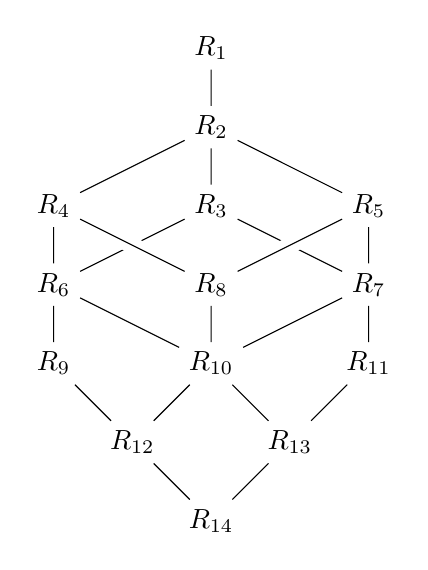
\begin{tikzpicture}
            \node (max) at (0,0) {$R_{14}$};
            \node (12) at (-1,1) {$R_{12}$};
            \node (13) at (1,1) {$R_{13}$};
            \node (9) at (-2,2) {$R_{9}$};
            \node (10) at (0,2) {$R_{10}$};
            \node (11) at (2,2) {$R_{11}$};
            \node (6) at (-2,3) {$R_{6}$};
            \node (8) at (0,3) {$R_{8}$};
            \node (7) at (2,3) {$R_{7}$};
            \node (4) at (-2,4) {$R_{4}$};
            \node (3) at (0,4) {$R_{3}$};
            \node (5) at (2,4) {$R_{5}$};
            \node (2) at (0,5) {$R_{2}$};
            \node (min) at (0,6) {$R_{1}$};
            \draw (min) -- (2) -- (4) -- (6) -- (9) -- (12) -- (max)
            (2) -- (5) -- (7) -- (11) -- (13) -- (max)
            (2) -- (3) -- (6) -- (10) -- (12)
            (3) -- (7) -- (10) -- (13)
            (8) -- (10);
            \draw[preaction={draw=white, -,line width=6pt}] (4) -- (8) -- (5);
        \end{tikzpicture}
    $$
\end{ex}

\newpage
\subsubsection*{Relaci\'on entre el conjunto de shuffles y el producto tensorial}
En este apartado veremos como relacionamos el conjunto de shuffles con el producto tensorial de cualquier par de \'arboles.
\begin{lema}
    Para todo shuffle $R_i$ de $S$ y $T$ tenemos un monomorfismo
    $$
        \xymatrix{
            m\colon\Omega[R_i] \ar@{>->}[r] & \Omega[S]\otimes\Omega[T]
        }
    $$
    El subconjunto dendroidal, que viene dado por la im\'agen de este monomorfismo, lo denotaremos $m(R_i)$.
\end{lema}
\begin{proof}
    Los v\'erties del conjunto dendroidal $\Omega[R_i]$ son las aristas del \'arbol $R_i$. La funci\'on $m$ env\'ia aristas nombradas como $(a,\text{ }x)$ en $R_i$ a la arista con el mismo nombre en $\Omega[S]\otimes\Omega[T]$.
    Vemos que es un monomorfismo.
    No entiendo.
\end{proof}
\begin{corol}
    Para todo objeto $T$ y $S$ en $\Omega$, tenemos que
    $$
        \Omega[S]\otimes\Omega[T] = \bigcup_{i=1}^{N} m(R_i)
    $$
    donde la uni\'on recorre todos los posibles shuffles de $S$ y $T$.
\end{corol}


\subsection{Shuffle de \'arboles en Python}
\newpage
% --- Acaba sección 4 ----------------------

% ------------------------------------------

% --- Empieza sección 5 --------------------
\section{Conclusiones}
\newpage
% --- Acaba sección 5 ----------------------

% --- Acaban las secciones -----------------

% --- Empieza la bibliografía ---
\begin{thebibliography}{25}
    \bibitem{pari} Batut, C.; Belabas, K.; Bernardi, D.; Cohen, H.; Olivier, M.: User's guide to \textit{PARI-GP},  \newline \texttt{pari.math.u-bordeaux.fr/pub/pari/manuals/2.3.3/users.pdf}, 2000.
    \bibitem{cw} Chen, J. R.; Wang, T. Z.: On the Goldbach problem, \textit{Acta Math. Sinica}, 32(5):702-718, 1989.
    \bibitem{desh} Deshouillers, J. M.: Sur la constante de $\check{\text{S}}\text{nirel}^{\prime} \text{man}$, \textit{S\'eminaire Delange-Pisot-Poitou, 17e ann\'ee: (1975/76), Th\'eorie des nombres: Fac. 2, Exp. No.} G16, p\'ag. 6, Secr\'etariat Math., Paris, 1977.
    \bibitem{derz} Deshouillers, J. M.; Effinger, G.; te Riele, H.; Zinoviev, D.: A complete Vinogradov 3-primes theorem under the Riemann hypothesis, \textit{Electron. Res. Announc. Amer. Math. Soc.}, 3:99-104, 1997.
    \bibitem{dick} Dickson, L. E.: \textit{History of the theory of numbers. Vol. I: Divisibility and primality}, Chelsea Publishing Co., New York, 1966.
    \bibitem{hl} Hardy, G. H.; Littlewood, J. E.: Some problems of \textquoteleft Partitio numerorum\textquoteright; III: On the expression of a number as a sum of primes, \textit{Acta Math.}, 44(1):1-70, 1923.
    \bibitem{hara} Hardy, G. H.; Ramanujan, S.: Asymptotic formulae in combinatory analysis, \textit{Proc. Lond. Math. Soc.}, 17:75-115, 1918.
    \bibitem{haw} Hardy, G. H.; Wright, E. M.: \textit{An introduction to the theory of numbers}, 5a edici\'on, Oxford University Press, 1979.
    \bibitem{minarc} Helfgott, H. A.: Minor arcs for Goldbach's problem, \newline \texttt{arXiv:1205.5252v4 [math.NT]}, diciembre de 2013.
    \bibitem{majarc} Helfgott, H. A.: Major arcs for Goldbach's problem, \newline \texttt{arXiv:1305.2897v4 [math.NT]}, abril de 2014.
    \bibitem{istrue} Helfgott, H. A.: The ternary Goldbach conjecture is true, \newline \texttt{arXiv:1312.7748v2 [math.NT]}, enero de 2014.
    \bibitem{HP} Helfgott, H. A.; Platt, D.: Numerical verification of the ternary Goldbach conjecture up to $8.875 \cdot 10^{30}$, \texttt{arXiv:1305.3062v2 [math.NT]}, abril de 2014.
    \bibitem{KPS} Klimov, N. I.; $\text{Pil}^{\prime} \text{tja}\breve{\imath}$, G. Z.; $\check{\text{S}}\text{eptickaja}$, T. A.: An estimate of the absolute constant in the Goldbach-$\check{\text{S}}\text{nirel}^{\prime} \text{man}$ problem, \textit{Studies in number theory, No. 4}, p\'ags. 35-51, Izdat. Saratov. Univ., Saratov, 1972.
    \bibitem{lw} Liu, M. C.; Wang, T.: On the Vinogradov bound in the three primes Goldbach conjecture, \textit{Acta Arith.}, 105(2):133-175, 2002.
    \bibitem{OSHP} Oliveira e Silva, T.; Herzog, S.; Pardi, S.: Empirical verification of the even Goldbach conjecture and computation of prime gaps up to $4\cdot10^{18}$, \textit{Math. Comp.}, 83:2033-2060, 2014.
    \bibitem{ram} Ramar\'e, O.: On $\check{\text{S}}\text{nirel}^{\prime} \text{man's}$ constant, \textit{Ann. Scuola Norm. Sup. Pisa Cl. Sci.}, 22(4):645-706, 1995.
    \bibitem{riva} Riesel, H.; Vaughan, R. C.: On sums of primes, \textit{Ark. Mat.}, 21(1):46-74, 1983.
    \bibitem{RS} Rosser, J. B.; Schoenfeld, L.: Approximate formulas for some functions of prime numbers, \textit{Illinois J. Math.}, 6:64-94, 1962.
    \bibitem{sch} Schnirelmann, L.: \"Uber additive Eigenschaften von Zahlen, \textit{Math. Ann.}, 107(1):649-690, 1933.
    \bibitem{tao} Tao, T.: Every odd number greater than $1$ is the sum of at most five primes, \textit{Math. Comp.}, 83:997-1038, 2014.
    \bibitem{ari} Travesa, A.: \textit{Aritm\`etica}, Co{\l}ecci\'o UB, No. 25, Barcelona, 1998.
    \bibitem{vau} Vaughan, R. C.: On the estimation of Schnirelman's constant, \textit{J. Reine Angew. Math.}, 290:93-108, 1977.
    \bibitem{vgn} Vaughan, R. C.: \textit{The Hardy-Littlewood method}, Cambridge Tracts in Mathematics, No. 125, 2a edici\'on, Cambridge University Press, 1997.
    \bibitem{vino} Vinogradov, I. M.: Sur le th\'eor\`eme de Waring, \textit{C. R. Acad. Sci. URSS}, 393-400, 1928.
    \bibitem{vin} Vinogradov, I. M.: Representation of an odd number as a sum of three primes, \textit{Dokl. Akad. Nauk. SSSR}, 15:291-294, 1937.
\end{thebibliography}
% --- Empieza la bibliografía ---

\end{document}

